
% {book} 		documento tipo 'book'
% [letterpaper] tamaño carta (216 x 279 mm)
% [12pt] 		letra a 12pt
% [openany]		los capitulos inician sin importar paginas pares o impares
% [oneside]		los margenes se acomodan para imprimir a una sola cara

\documentclass[letterpaper,10pt,openany,oneside,final]{book}



% {geometry}	Diseño de la región impresa
% [total]		Dimensiones {Ancho, Alto}
% [top]			Margen superior
% [left]		Margen izquierdo

\usepackage[left=3cm, top=2.5cm, right=2.5cm, bottom=2.5cm]{geometry}



% include		Incluye un archivo .tex
% {Packages}	Importa todos los paquetes a usar en este documento

%%%%%%%%%%%%%%%%%%%%%%%%%%%%%%%%%%%%%
% Paquete para símbolos matematicos %
%%%%%%%%%%%%%%%%%%%%%%%%%%%%%%%%%%%%%
\usepackage{amsmath,amssymb,amsfonts,latexsym,cancel} %paquetes para simbolos matematicos
\usepackage[utf8]{inputenc}     % codificación de entrada
\usepackage[T1]{fontenc}        % fundición de salida
\usepackage[spanish,es-noshorthands,es-tabla]{babel} %partición de palabras
%\usepackage[breaklinks=true]{hyperref} %enlaces


% UTILES
\usepackage{listingsutf8}
\usepackage{pdfpages}
\usepackage{comment}
\usepackage{float}
\usepackage{caption} 
\usepackage[shortlabels]{enumitem}
%\usepackage[x11names,table]{xcolor}
\usepackage[rtlf]{floatflt}
\usepackage{longtable, booktabs, multirow, multicol}



% GRAFICOS Y FIGURAS
\usepackage{graphicx} %insercción de graficos
\usepackage{pgf-pie}
\usepackage{subfigure}
\usepackage{wrapfig} %figuras flotantes


% TIKZ
\usepackage{tikz} 
\usepackage{tikz-uml}
\usetikzlibrary{arrows.meta}
\usetikzlibrary{trees}
\usetikzlibrary{positioning}
\usetikzlibrary{intersections}


% ALGUNAS CONFIGURACIONES
\usepackage{fancyhdr}
\pagestyle{myheadings} % permite modificar el estilo de los encabezados de página
\captionsetup[figure]{labelfont={bf,small},textfont={sl,normalsize},labelsep=period}
\captionsetup[table]{labelfont={bf,small},textfont={sl,normalsize},labelsep=period}



% {fontspec}	permite el uso de setmainfont
% {Arial}		Toma la letra Arial del sistema y la establece para el documento

\usepackage{fontspec}
%\setmainfont{Arial}

\setmainfont{Times New Roman}
\setsansfont{Arial}
%\setmonofont{Cambria}



% Interlineado 1.5
\usepackage{setspace}
\onehalfspacing
%\linespread{1.3}
% \renewcommand{\baselinestretch}{1.5} 




% Configuracion de listings
\include{Config_Listings}



% Formato de titulos
\usepackage{titlesec}

%\titleformat{\chapter}[display]{\large \textrm \bfseries}{\filcenter\chaptertitlename\ \thechapter}{6pt}{ \large\textrm\bfseries }
\titleformat
{\chapter}[display]
{\bfseries\Large}{\chaptertitlename\ \thechapter}{-\parskip}{\bfseries\Large}

\assignpagestyle{\chapter}{myheadings}


\titleformat*{\section}{\bfseries\large}
\titleformat*{\subsection}{\bfseries\normalsize}
\titleformat*{\subsubsection}{\bfseries\normalsize}
\titleformat*{\paragraph}{\bfseries\normalsize}

\titlespacing{\chapter}{0pt}{-2em}{\parskip}
\titlespacing{\section}{0pt}{\parskip}{-\parskip}
\titlespacing{\subsection}{0pt}{\parskip}{-\parskip}
\titlespacing{\subsubsection}{0pt}{\parskip}{-\parskip}

% Formato de la pagina, numeración en esquina superior izq
%\usepackage{etoolbox}
%\patchcmd{\chapter}{plain}{myheadings}{}{}


\begin{document}


% Inclusion de la portada
\includepdf{Anexos/Portada}

% Inclusion de la portada
\includepdf{Anexos/Aprobacion}

% Inclusion de la portada
\includepdf{Anexos/Autorizacion}

%Dra. Anamim V. Wong.
%Dra. Jehiely Belem H. C.  \& Ing. Rosel Muñoz López

%--------------------------------------------------------------------------------------------
\chapter*{Dedicatoria}
\thispagestyle{empty}
%\pagenumbering{Roman} % para comenzar la numeracion de paginas en numeros romanos

	\begin{flushright}
	\vfill
	\textbf{A NUESTROS PADRES, PROFESORES Y AMIGOS}\\
	\textit{Que nos han apoyado en nuestra trayectoria universitaria, en especial a aquellos\\ que nos abrieron las puertas y compartieron sus conocimientos.}
	\vfill
\end{flushright}

\chapter*{Agradecimientos}
\thispagestyle{empty}
\vfill
{\flushright \textbf{Nuestros Padres}\\}

\textit{Por su amor, trabajo y sacrificio en todos estos años, gracias a ustedes hemos logrado llegar hasta aquí y convertirnos en lo que somos. Ha sido un orgullo y privilegio ser sus hijos, son los mejores padres.}
\newline

{\flushright \textbf{Dra. Anamim V. Wong.\\}}

\textit{Asesora de tesis, deseamos reconocer su valiosa guía, trabajo y dedicación permanente y continua al presente trabajo, así como sus sugerencias y observaciones, siempre inteligentes y oportunas.}
\newline

{\flushright \textbf{Dra. Jehiely Belem H. C.  \& Ing. Rosel Muñoz López}\\}

\textit{Por todas sus aportaciones para el desarrollo de este documento, así como reconocer todos los conocimientos que han logrado transmitirnos en las innumerables horas que hemos pasado juntos trabajando en los últimos años, siempre les estaremos agradecidos.}
\newline
\vfill






%-----------------------------------------------------------------------------------------------------------------------------

\begin{comment}


\newpage
{\Large \textbf{DEDICATORIA}}
\thispagestyle{empty}
\vspace{2\parsep}


{\flushright \textbf{A NUESTROS PADRES, PROFESORES Y AMIGOS\\} }
\textit{Que nos han apoyado en nuestra trayectoria universitaria, en especial a aquellos que nos abrieron las puertas y compartieron sus conocimientos.}





\vspace{4cm}
{\Large \textbf{AGRADECIMIENTOS}}
\vspace{2\parsep}

{\flushright \textbf{NUESTROS PADRES}\\}

\textit{Por su amor, trabajo y sacrificio en todos estos años, gracias a ustedes hemos logrado llegar hasta aquí y convertirnos en lo que somos. Ha sido un orgullo y privilegio ser sus hijos, son los mejores padres.}
\newline

{\flushright \textbf{NUESTRA ASESORA\\}}

\textit{Asesora de tesis, deseamos reconocer su valiosa guía, trabajo y dedicación permanente y continua al presente trabajo, así como sus sugerencias y observaciones, siempre inteligentes y oportunas.}
\newline

{\flushright \textbf{NUESTROS REVISORES}\\}

\textit{Por todas sus aportaciones para el desarrollo de este documento, así como reconocer todos los conocimientos que han logrado transmitirnos en las innumerables horas que hemos pasado juntos trabajando en los últimos años, siempre les estaremos agradecidos.}
\newline
\end{comment}

% Inclusion de la portada
\includepdf{Anexos/Contraportada}

% :::::::::::::::::::::::::::::::::::::::::::::::::
%  Genera la lista de contenidos, figuras y tablas
% :::::::::::::::::::::::::::::::::::::::::::::::::

\pagenumbering{Roman}
\tableofcontents

%\clearpage
%\addcontentsline{toc}{section}{\listfigurename}
\listoffigures

%\clearpage
%\addcontentsline{toc}{section}{\listtablename}
\listoftables






\setlength{\parindent}{0pt}
\setlength{\parskip}{1ex plus 0.5ex minus 0.2ex}
\setlength{\itemsep}{0mm}
%\setlength{\baselineskip}{1.35\baselineskip}

\chapter{Generalidades del proyecto}

\section{Introducción}

En la ciudad de Tapachula Chiapas el índice demográfico se encuentra en constante crecimiento por lo que la movilidad urbana o el total de desplazamientos que se realizan en la ciudad es un factor importante que afecta el congestionamiento vehicular.

La adecuada operación de los semáforos en las intersecciones es otro factor importante, debido a que, son estos quienes dirigen el flujo del tráfico. Desafortunadamente los semáforos convencionales tienen asignados tiempos fijos para el cambio de luces, esto a menudo ocasiona largos tiempos de espera innecesarios.  

En el presente documento se redacta el desarrollo de un sistema “inteligente” que hará uso de herramientas y técnicas de Inteligencia Artificial para la sincronización de los semáforos.

El sistema desarrollado será capaz de gestionar los semáforos de una intersección de 4 vías con doble sentido. Para esto el sistema reaccionará a variables de su entorno como:

{\setlength{\baselineskip}{0.7\baselineskip}
\begin{itemize}
	\item Cantidad de carriles de las avenidas.
	\item Congestión de toda la intersección.
\end{itemize}}

Con este proyecto se espera alentar a los alumnos a que sigan investigando sobre el tema, ya que una buena gestión de tráfico no solo favorece la movilidad vehicular, sino también, disminuye la emisión de gases contaminantes (producto de los autos varados en los cruces), lo cual es un tema muy importante actualmente debido al calentamiento global.

\section{Descripción de la empresa}

En el presente capítulo se describen los datos del “Instituto Tecnológico de Tapachula” lugar en donde se desarrolló el proyecto, también se encuentra información acerca de la localización y el área en donde se elaboró el proyecto.

\subsection*{Nombre o Razón Social}
Instituto Tecnológico de Tapachula.

\subsection*{Breve descripción de la empresa}
El instituto tecnológico de Tapachula es una institución educativa perteneciente al sistema nacional de institutos tecnológicos, que a su vez forma parte de la dirección general de educación superior tecnológica. Cuenta con las siguientes carreras: 
\begin{multicols}{2}
{\setlength{\baselineskip}{0.7\baselineskip}\begin{itemize}
	\item Ing. Civil
	\item Ing. Industrial
	\item Ing. Química
	\item Ing. Electromecánica
	\item Ing. En Sistemas Computacionales.
	\item Ing. En Gestión Empresarial
\end{itemize}}
\end{multicols}

\subsection*{Antecedentes del ITT}

El Instituto Tecnológico de Tapachula pertenece al Tecnológico Nacional de México, que está integrada por 218 Institutos Tecnológicos y Centros Especializados, distribuidos en el territorio Mexicano. De ellos, 110 son de carácter federal, entre los que destacan 104 Institutos Tecnológicos Industriales, dos Centros Especializados y cuatro Centros de Desarrollos Tecnológico. A lo mismo se unen 108 Tecnológicos Descentralizados, los cuales han servido al país durante más de 57 años de vida, siempre con el compromiso de hacer el mejor de sus esfuerzos; procurando que la educación que se imparten en dichas Instituciones Educativas responda a las exigencias de los más altos estándares de calidad educativa.

Atendiendo a las líneas de desarrollo regional para asegurar la pertenecía de los planes y programas de estudio; conscientes de que representan una vía de desarrollo, de esperanza, de inclusión y de movilidad social para los jóvenes de la provincia mexicana. El 16 de Mayo de 1983, el Instituto Tecnológico de Tapachula, abre sus puerta a la superación profesional a través de la carrera de Ingeniería Civil, además continua a 148 alumnos con nivel medio superior con una carrera terminal en tecnólogos en construcción y tecnólogos en electrotecnia, de igual manera absorbe a la población de nivel de licenciatura del CeRETI, en las carreras de Ingeniería Industrial en alimentos e Ingeniería Civil, permitiendo a los alumnos de ésta última cambiarse al plan de tecnológico.

Se autoriza el 15 de Noviembre de 1984; la apertura de la carrera de ingeniería Química, inscribiéndose para el semestre inicial, Septiembre 85 - Febrero 86, un total de 73 alumnos, en ese entonces el C. Ing. Jorge Elí Castellanos Martínez, como director del plantel, fue el encargado de darles la bienvenida.

El 29 de Mayo de 1985, siendo el director del plantel el C. Jorge Carlos García Revilla, se autoriza la carrera de Ingeniería Industrial, matriculando 54 alumnos para el semestre Septiembre 86 - Febrero 87. Uno de los objetivos primordiales del instituto es brindar a la juventud estudiosa del estado de Chiapas, la oportunidad de formación y superación profesional a través de las diferentes carreras que se imparten, ampliando la oferta educativa; es por ello que en 1990 se crea la carrera de licenciatura en Informática, con una población de 70 alumnos, y es el C. Ing. Víctor Manuel Ibarra Balderas, director del plantel, el encargado de darle la bienvenida a los alumnos de nuevo ingreso.

Un nuevo estudio sobre la demanda educativa en el estado, muestra la necesidad de proporcionar una nueva opción de formación profesional, en respuesta a ello el 28 de Enero de 1993, siendo el director el C. Ing. José Luis Méndez Navarro, se autoriza la carrera de Ingeniería Electromecánica, iniciándose en el mes de Agosto del mismo año con una población de 29 alumnos. Las necesidades de la región, así como un nuevo estudio de expectativas, dieron como resultado que el 18 de Junio del 2002, autorizaran la carrera de Ingeniería en Sistemas computacionales. El C. M.A. Juan Amado Rueda Ibarra, como máxima autoridad de la institución les da la bienvenida, el 18 de Agosto de 2003, a los 45 miembros de la primera generación de esta carrera. También comparte el conocimiento científico y tecnológico con el público en general, a través de su programa de educación continua, el cual está compuesto por diferentes cursos de interés general, destacándose los del idioma de idioma de inglés en sus diferentes niveles. Los programas de servicio social y residencia profesional han permitido atender en las peticiones a más de 150 Instituciones municipales, estatales y federales de los sectores públicos y privado.

Como parte del compromiso que se tiene con la sociedad como institución educativa, el Instituto Tecnológico de Tapachula orgullosamente ha obtenido la certificación del proceso educativo de acuerdo a la norma ISO 9001:2000, cuyo certificado RSGC 247 le fue entregado el 2 de Octubre de 2006, y que en nombre de los trabajadores del Instituto Tecnológico lo recibió el Ing. Herman Calderón Pineda, en ese entonces director.

Tapachula, Abril 14.- Con entusiasmo fue recibida la noticia por la “comunidad tecnológica” la designación del maestro en ciencias de la administración, Miguel Cid del Prado Martínez, como nuevo Director del Instituto Tecnológico de Tapachula (ITT); designación realizada con fecha 24 de marzo del año en curso por el doctor Carlos Alfonso García Ibarra, Director General de Educación Superior Tecnológica de la SEP.

Correspondió al Doctor Héctor Francisco Macías Díaz, Director de Capacitación y Desarrollo de la DGEST, quien en calidad de representante del Director General hizo la presentación del nuevo director, Del Prado Martínez, quien -dijo- venía fungiendo como  subdirector de los servicios administrativos del Instituto Tecnológico de Tuxtla Gutiérrez, donde además desempeñó los cargos de profesor de licenciatura y posgrado, fue Jefe de la División de Estudios de Posgrado e Investigación, Jefe del Departamento de Ingeniería Química, Coordinador de la Especialización en Ingeniería Ambiental, Coordinador de la Maestría en Ciencias de la Administración y Coordinador de Educación a Distancia.

El Ing. Pedro Ancheyta Bringas, en su calidad de Director del Instituto Tecnológico de Tapachula, manifestó el doble compromiso que para él representa la nueva encomienda: como lealtad y responsabilidad por ser egresado del Tecnológico de Tapachula, pero hoy asume dicha función con todos los deseos de sumarse al trabajo”


El 5 de Abril del 2017.- El Maestro Manuel Quintero Quintero Director General del Tecnológico Nacional de México (TecNM), nombró a la maestra Rosa Aidé Domínguez Ochoa como nueva Directora del Instituto Tecnológico de Tapachula, quien asumió sus funciones con esta fecha.


Actualmente, se cuenta con una población estudiantil de: 1 mil 801 alumnos, distribuidos en las diferentes carreras. 

El Instituto Tecnológico de Tapachula Nº 51 se dedica a contribuir a la conformación de una sociedad más justa, humana y con amplia cultura científico-tecnológica, mediante un sistema integrado de educación superior tecnológica, equitativo en su cobertura y de alta calidad.

El Departamento de Sistemas y Computación del Instituto Tecnológico de Tapachula su giro es público.\\


\parbox[t]{0.48\textwidth}{
{\setlength{\baselineskip}{1.5\baselineskip}
\textbf{Misión}\\
Contribuir a la conformación de una sociedad más justa, humana y con amplia cultura científico-tecnológica, mediante un sistema integrado de educación superior tecnológica, equitativo en su cobertura y de alta calidad.\par}
}\hfill
\parbox[t]{0.48\textwidth}{
{\setlength{\baselineskip}{1.3\baselineskip}
\textbf{Visión}\\
El Sistema Nacional de Institutos Tecnológicos se consolidará como un sistema de educación superior tecnológica de vanguardia, así como uno de los soportes fundamentales del desarrollo sostenido, sustentable y equitativo de la nación y del fortalecimiento de su diversidad cultural.\par}
}

\subsection*{Valores}
\begin{multicols}{3}
\begin{itemize}
\item El ser humano
\item El liderazgo
\item La calidad
\item El espíritu de servicio
\item El trabajo en equipo
\item El alto desempeño
\end{itemize}
\end{multicols}
%\subsection*{Políticas de Calidad}

\subsection*{Organigrama}

La figura~\ref{fig:organigrama} muestra el organigrama.

\begin{figure}[H]
\begin{tikzpicture}[edge from parent fork down, sibling distance=15mm, level distance=15mm,
every node/.style={fill=gray!10,rounded corners,align=center},
primary/.style={text width=2.5cm, font=\scriptsize , inner sep=3pt },
depto/.style={anchor=north, minimum height=4.2em, text width=1.8cm, font=\scriptsize},
depto2/.style={anchor=north, minimum height=4em, text width=2.5cm, font=\scriptsize},
proyec/.style={anchor=north, minimum height=4em, text width=1.8cm, font=\scriptsize},
office/.style={anchor=west, minimum height=3.2em, text width=2.2cm, font=\scriptsize},
line/.style={draw, semithick }]
\node[primary] (direc) {\textsc{Dirección}};

\node[primary, anchor=east] at (-2,-0.7) (cdp) {\textsc{Comité de planeación}};
\node[primary, anchor=west,text width=5cm] at ( 2,-0.7) (comgtv) {\textsc{Comité de gestión tecnológica y vinculación}};

\node [primary] at (-6,-2.1) (subv) {\textsc{Subdirección de planeación y vinculación}};
\node [primary] at (0,-2) (suba) {\textsc{Subdirección académica}};
\node [primary] at (6,-2.1) (subs) {\textsc{Subdirección de servicios administrativos}};

\node [primary] at (-6,-3.1) (conedit) {\textsc{Consejo editorial}};
\node [primary] at (2,-3) (comadm) {\textsc{Comité académico}};	

\node [depto] at (-6.6,-4.2) (depcb) {\textsc{Depto. de ciencias básicas}};
\node [depto] at (-4.4,-4.2) (depsc) {\textsc{Depto. de sistemas y computación}};
\node [depto] at (-2.2,-4.2) (depct) {\textsc{Depto. de ciencias de la tierra}};
\node [depto] at (0,-4.2) (depii) {\textsc{Depto. de ingeniería industrial}};
\node [depto] at (2.2,-4.2) (depqb) {\textsc{Depto. de ingenieria quimica y bioquimica}};
\node [depto] at (4.4,-4.2) (depea) {\textsc{Depto. de ciencias económico administrativas}};
\node [depto] at (6.6,-4.2) (depep) {\textsc{División de estudios profesionales}};

\node [proyec] at (-6.6,-6.1) (procb) {\textsc{Proyectos de docencia investigación y vinculación}};
\node [proyec] at (-4.4,-6.1) (prosc) {\textsc{Proyectos de docencia investigación y vinculación}};
\node [proyec] at (-2.2,-6.1) (proct) {\textsc{Proyectos de docencia investigación y vinculación}};
\node [proyec] at (0,-6.1) (proii) {\textsc{Proyectos de docencia investigación y vinculación}};
\node [proyec] at (2.2,-6.1) (proqb) {\textsc{Proyectos de docencia investigación y vinculación}};
\node [proyec] at (4.4,-6.1) (proea) {\textsc{Proyectos de docencia investigación y vinculación}};
\node [proyec] at (6.6,-6.1) (proep) {\textsc{Proyectos de docencia investigación y vinculación}};

\node [shape=circle, draw, inner sep=1pt] at (0,-8.5) (conector) {{\scriptsize 1}};

\node [depto2] at (-6,-9) (depdp) {\textsc{Depto. de desarrollo y programación}};
\node [depto2] at (-3,-9) (depgv) {\textsc{Depto. de gestión y vinculación}};
\node [depto2] at (0,-9) (depae) {\textsc{Depto. de actividades extraescolares}};
\node [depto2] at (3,-9) (depci) {\textsc{Centro de información}};
\node [depto2] at (6,-9) (depse) {\textsc{Depto. de servicios escolares}};

\node [office] at (-7,-12) (officea1) {\textsc{Oficina de desarrollo institucional}};
\node [office] at (-4,-12) (officea2) {\textsc{Oficina de prácticas y promoción profesional}};
\node [office] at (-1,-12) (officea3) {\textsc{Oficina de promoción cultural}};
\node [office] at (2,-12) (officea4) {\textsc{Oficina de control escolar}};
\node [office] at (5,-12) (officea5) {\textsc{Oficina de organización bibliográfica}};

\node [office] at (-7,-13.5) (officeb1) {\textsc{Oficina de programación y evaluación presupuestaria}};
\node [office] at (-4,-13.5) (officeb2) {\textsc{Oficina de servicio social y desarrollo comunitario}};
\node [office] at (-1,-13.5) (officeb3) {\textsc{Oficina de promoción deportiva}};
\node [office] at (2,-13.5) (officeb4) {\textsc{Oficina de servicios estudiantiles}};
\node [office] at (5,-13.5) (officeb5) {\textsc{Oficina de servicios a usuario}};

\node [office] at (-7,-15) (officec1) {\textsc{Oficina de servicios externos}};
\node [office] at (-4,-15) (officec2) {\textsc{Oficina de construcción y equipamiento}};
\node [office] at (-1,-15) (officec3) {\textsc{Oficina de comunicación y difusión}};
%\node [office] at (2,-15) (depci) {\textsc{Oficina de servicios estudiantiles}};
\node [office] at (5,-15) (officec5) {\textsc{Oficina de servicios especializados}};

\begin{scope}[every path/.style=line]

\path (direc) -- (suba);
\path (0,-0.7) -- (cdp);
\path (0,-0.7) -- (comgtv);


\path (direc) +(0,-1.4) -| (subv);
\path (direc) +(0,-1.4) -| (subs);

\path (0,-3) -- (comadm);

\path (conedit.west) -- ++(-0.4,0) -- ++(0,-4.9) -- ++(15.5,0) |- (subs.east);
\path (conedit.west) ++(-0.4,0) |- (subv.west);

\path (suba) -- ++(0,-2) -| (depcb);
\path (suba)  ++(0,-2) -| (depsc);
\path (suba)  ++(0,-2) -| (depct);
\path (suba)  ++(0,-2) -| (depii);
\path (suba)  ++(0,-2) -| (depqb);
\path (suba)  ++(0,-2) -| (depea);
\path (suba)  ++(0,-2) -| (depep);

\path (depcb) -- (procb);
\path (depsc) -- (prosc);
\path (depct) -- (proct);
\path (depii) -- (proii);
\path (depqb) -- (proqb);
\path (depea) -- (proea);
\path (depep) -- (proep);

%segunda parte
\path (conector.south) -- ++(0,-0.2);
\path (conector.south) ++(0,-0.2) -| (depdp);
\path (conector.south) ++(0,-0.2) -| (depgv);
\path (conector.south) ++(0,-0.2) -| (depae);
\path (conector.south) ++(0,-0.2) -| (depci);
\path (conector.south) ++(0,-0.2) -| (depse);

\path (depdp.south) -- ++(0,-0.4) -- ++(-1.2,0);
\path (depdp.south) ++(0,-0.4) ++(-1.2,0) |- (officea1.west);
\path (depdp.south) ++(0,-0.4) ++(-1.2,0) |- (officeb1.west);
\path (depdp.south) ++(0,-0.4) ++(-1.2,0) |- (officec1.west);

\path (depgv.south) -- ++(0,-0.4) -- ++(-1.2,0);
\path (depgv.south) ++(0,-0.4) ++(-1.2,0) |- (officea2.west);
\path (depgv.south) ++(0,-0.4) ++(-1.2,0) |- (officeb2.west);
\path (depgv.south) ++(0,-0.4) ++(-1.2,0) |- (officec2.west);

\path (depae.south) -- ++(0,-0.4) -- ++(-1.2,0);
\path (depae.south) ++(0,-0.4) ++(-1.2,0) |- (officea3.west);
\path (depae.south) ++(0,-0.4) ++(-1.2,0) |- (officeb3.west);
\path (depae.south) ++(0,-0.4) ++(-1.2,0) |- (officec3.west);

\path (depci.south) -- ++(0,-0.4) -- ++(-1.2,0);
\path (depci.south) ++(0,-0.4) ++(-1.2,0) |- (officea4.west);
\path (depci.south) ++(0,-0.4) ++(-1.2,0) |- (officeb4.west);
%\path (depci.south) ++(0,-0.4) ++(-1.2,0) |- (officec2.west);

\path (depse.south) -- ++(0,-0.4) -- ++(-1.2,0);
\path (depse.south) ++(0,-0.4) ++(-1.2,0) |- (officea5.west);
\path (depse.south) ++(0,-0.4) ++(-1.2,0) |- (officeb5.west);
\path (depse.south) ++(0,-0.4) ++(-1.2,0) |- (officec5.west);
\end{scope}
\end{tikzpicture}
\caption{Organigrama del Instituto Tecnológico de Tapachula}\label{fig:organigrama}
\end{figure}

%\begin{figure}[H]
%\centering
%\includegraphics[width=12cm,height=10cm]{sources/organigramaA.png}
%\caption{Organigrama-A del Instituto Tecnológico de Tapachula}\label{fig:ogngmA}
%\end{figure}

%\begin{figure}[H]
%\centering
%\includegraphics[width=14cm,height=6cm]{sources/organigramaB.png}
%\caption{Organigrama-B del Instituto Tecnológico de Tapachula}\label{fig:ogngmB}
%\end{figure}

\newpage

\subsection*{Ubicación del Instituto Tecnológico}
El Instituto Tecnológico de Tapachula, se encuentra ubicado en el Km. 2 Carretera a Puerto Madero. C.P. 30700 Tapachula, Chiapas.

%
\subsection*{Macro-localización}

La figura~\ref{fig:macroloc} muestra una vista aérea de la Macro Localización.

\begin{figure}[H]
\centering
\includegraphics[scale=0.8]{sources/macrolocalizacion.png}
\caption{Macro Localización del Instituto Tecnológico de Tapachula}\label{fig:macroloc}
\end{figure}

%\newpage
\pagebreak
\subsection*{Ubicación del Área en donde se elaboró el proyecto}

El proyecto “implementación de un algoritmo de sincronización de semáforos usando inteligencia artificial” se desarrolla en el Departamento de Sistemas y Computación, en el área de Investigación y Desarrollo del Instituto Tecnológico de Tapachula, ubicado en el edificio “Centro de información”.

\begin{figure}[!hb]
\centering
\includegraphics[scale=0.8]{sources/microlocalizacion.png}
\caption{Micro Localización del Instituto Tecnológico de Tapachula}\label{fig:microloc}
\end{figure}

\subsection*{Características del Área o Departamento}

% subsection subsection_name (end)
\subsubsection*{Departamento de Investigación y Desarrollo}

{\setlength{\baselineskip}{0.8\baselineskip}
\begin{enumerate}
\item Planear, coordinar y evaluar las actividades de docencia, investigación y vinculación de las áreas correspondientes a sistemas y computación que se imparten en el Instituto Tecnológico de Tapachula, de conformidad a las normas y lineamientos establecidos por la secretaria de educación pública.

\item Elaborar el programa operativo anual y el anteproyecto de presupuesto y los procedimientos establecidos.

\item Aplicar la estructura orgánica autorizada para el departamento y los procedimientos establecidos 

\item  Coordinar con las divisiones de estudios profesionales y postgrado e investigación, y la aplicación de los programas de estudio y con el departamento de desarrollo académico los materiales y apoyo didáctico de las asignaturas correspondientes a las áreas de sistemas y computación que se imparten en el Instituto Tecnológico y controlar su desarrollo

\item Coordinar los proyectos de investigación educativa, científica y tecnológica en las áreas de sistemas y computación que se llevan a cabo en el Instituto Tecnológico y controlar su desarrollo 

\item Coordinar los proyectos de producción académica y de investigación científica y tecnológica en las áreas de sistemas y computación relacionas con la vinculación del instituto tecnológico con el sector productivo de bienes, servicios de la región y controlar su desarrollo.

\item Proponer a la subdirección académica el desarrollo de cursos y eventos que propicien la superación y actualización profesional del personal docente de las áreas de sistemas y computación en el Instituto Tecnológico.

\item Apoya a la división de estudios profesionales en el proceso de titulación de los alumnos del instituto.

\item Supervisar y evaluar el funcionamiento del departamento y con base en los resultados, proponer las medidas que mejoren su operación.

\item Coordinar las actividades del departamento con las demás áreas den la subdirección académica 

\item Presentar reportes periódicos de las actividades desarrolladas a la subdirección académica.

\end{enumerate}
}
\subsubsection*{Funciones}

Planear, organizar, dirigir, controlar y evaluar de acuerdo con las normas y lineamientos establecidos, las actividades de docencia, investigación y vinculación del instituto tecnológico. Elaborar el programa operativo anual y el anteproyecto propuesto a la subdirección del instituto tecnológico para lo conducente. Coordinar las actividades de la subdirección con las demás áreas para los cumplimientos de los objetivos del instituto tecnológico.


\chapter{Descripción del proyecto}
En este capítulo se presenta la descripción del proyecto “Implementación de un algoritmo de sincronización de semáforos usando inteligencia artificial”, en donde se da a conocer la razón por la cual se decidió desarrollar la investigación, así como también, los objetivos que se deben cumplir, los problemas que resuelve el mismo, los alcances y limitaciones que se presentan.

\section{Problemas a resolver}
En la ciudad de Tapachula, no existen semáforos inteligentes que sean capaces de resolver los problemas que todos los días se presentan a consecuencia de la gran cantidad de automóviles que circulan en las calles.

Debido a ello en un futuro se pretende la creación de estos semáforos, pero para su desarrollo es necesario el uso de un algoritmo de sincronización que permita la comunicación entre semáforos de avenidas intersectadas y decida el estatus de cada uno de ellos.

\section{Alcances y Limitaciones}
\subsection*{Alcances del proyecto}
\begin{itemize}
\item El algoritmo contará con un tiempo de respuesta en el orden de milisegundos para su implementación en el control de semáforos.
\end{itemize}

\subsection*{Limitaciones del proyecto}
\begin{itemize}
\item El algoritmo sólo comunicará los semáforos de cuatro avenidas que se intersectan.
\end{itemize}

\section{Objetivos}

\subsection*{Objetivo general}
Implementar un algoritmo de sincronización de semáforos utilizando inteligencia artificial.

\subsubsection*{Objetivos específicos}
\begin{itemize}
\item Seleccionar la técnica de inteligencia artificial que resuelva la sincronización entre los semáforos.
\item Implementar un algoritmo que use la técnica seleccionada y que determine el estatus de cada semáforo y el tiempo que permanecerá dicho estatus.
\end{itemize}

\section{Justificación}
Las ciudades son lugares en donde se realiza una alta actividad económica y en donde transportarse forma parte de la vida cotidiana de las personas; mientras que para las empresas representa una parte esencial de su operación diaria. Estos factores hacen que en las calles principales de la ciudad exista tráfico vehicular y aumente la contaminación del medio ambiente, lo cual es perjudicial para las personas y el ambiente mismo.

Tomando en cuenta los puntos antes mencionados, se considera importante, que en la ciudad de Tapachula, Chiapas, se debe de contar con un sistema inteligente que permita controlar de manera eficiente el flujo vehicular y peatonal, para lograr este objetivo será necesario que el sistema sea capaz de realizar el conteo de los automóviles de una forma rápida, logrando con ello tener un control que permita administrar el tiempo de espera para ceder el paso a los automóviles y así mismo a los peatones.


\chapter{Descripción del proyecto}

En este capítulo se presenta la descripción del proyecto “Implementación de un algoritmo de sincronización de semáforos usando inteligencia artificial”, en donde se da a conocer la razón por la cual se decidió desarrollar la investigación, así como también, los objetivos que se deben cumplir, los problemas que resuelve el mismo, los alcances y limitaciones que se presentan.

\section{Problemas a resolver}
En la ciudad de Tapachula, no existen semáforos inteligentes que sean capaces de resolver los problemas que todos los días se presentan a consecuencia de la gran cantidad de automóviles que circulan en las calles.

Debido a ello en un futuro se pretende la creación de estos semáforos, pero para su desarrollo es necesario el uso de un algoritmo de sincronización que permita la comunicación entre semáforos de avenidas intersectadas y decida el estatus de cada uno de ellos.

\section{Alcances y limitaciones}
\subsection*{Alcances del proyecto}
\begin{itemize}
\item El algoritmo contará con un tiempo de respuesta en el orden de milisegundos para su implementación en el control de semáforos.
\end{itemize}

\subsection*{Limitaciones del proyecto}
\begin{itemize}
\item El algoritmo solo comunicará los semáforos de cuatro avenidas que se intersectan.
\end{itemize}

\section{Objetivos}

\subsection*{Objetivo general}
Implementar un algoritmo de sincronización de semáforos utilizando inteligencia artificial.

\subsection*{Objetivos específicos}
\begin{itemize}
\item Seleccionar la técnica de inteligencia artificial que resuelva la sincronización entre los semáforos.
\item Implementar un algoritmo que use la técnica seleccionada y que determine el estatus de cada semáforo y el tiempo que permanecerá dicho estatus.
\end{itemize}

\section{Justificación}
Las ciudades son lugares en donde se realiza una alta actividad económica y en donde transportarse forma parte de la vida cotidiana de las personas; mientras que para las empresas representa una parte esencial de su operación diaria. Estos factores hacen que en las calles principales de la ciudad exista tráfico vehicular y aumente la contaminación del medio ambiente, lo cual es perjudicial para las personas y el ambiente mismo.

Tomando en cuenta los puntos antes mencionados, se considera importante, que en la ciudad de Tapachula, Chiapas, se debe de contar con un sistema inteligente que permita controlar de manera eficiente el flujo vehicular y peatonal, para lograr este objetivo será necesario que el sistema sea capaz de realizar el conteo de los automóviles de una forma rápida, logrando con ello tener un control que permita administrar el tiempo de espera para ceder el paso a los automóviles y así mismo a los peatones.


\chapter{Desarrollo}

En este capítulo se describe el desarrollo del sistema en general: la selección de la técnica, el desarrollo de la técnica seleccionada y la selección del lenguaje de programación.

A continuación, en la \textbf{sección \ref{section:selecciontecnica}} se describe, a manera de resumen: las diferentes técnicas tomadas en cuenta durante la investigación y los porqués de la técnica seleccionada.

Después en la \textbf{sección \ref{section:desarrolloFIS}}, se describe el proceso de diseño del \textit{Sistema de Inferencia Difuso} bajo una metodología de mejora iterativa. El sistema tiene como objetivo calcular el tiempo de la fase en verde de un semáforo, que mediante la estructura propuesta y un preprocesamiento de los datos, permitirá gestionar diferentes tipos de intersecciones.

Posteriormente en la \textbf{sección \ref{section:desarrolloAlgoritmo}} se modela, mediante diagramas UML, la arquitectura del software desarrollado. El resultado es una micro-librería que permite \emph{expresar las variables y reglas del sistema difuso en notación de objetos}. Además, se modela la estructura propuesta para integrar la técnica seleccionada, a un sistema de control (a un algoritmo de sincronización) de semáforos y así, posibilitar la aplicación del sistema a una intersección con número no-estático de avenidas y fases.

\section{Preliminares}
Antes de continuar con el diseño del sistema, se considera adecuado aclarar algunos puntos acerca de:

\paragraph{El enfoque}presentado en este proyecto difiere con el resto en que, fue diseñado para ser embebido dentro de un algoritmo de sincronización de semáforos más general, de esta manera la tarea del \textit{FIS} se centra en determinar el tiempo en verde, dejando los detalles de sincronización en manos de un segundo algoritmo (también propuesto y desarrollado en este proyecto).

%El segundo algoritmo se encarga no solo del \emph{pre} y \emph{post} procesamiento de los datos de entrada y salida, sino que también define un marco de trabajo para la implementación final por parte del usuario final, valga la redundancia.

\paragraph{El pre-procesamiento} de los datos permite, mediante un proceso matemático sencillo, adaptar el \emph{FIS} propuesto a cruces con un número arbitrario de avenidas y fases, por ejemplo, intersecciones de: 2 avenidas y 2 fases, 4 avenidas y 2 fases o 4 avenidas y 4 fases. De esta manera se logra integrar una técnica de inteligencia artificial con un segundo algoritmo para la sincronización de semáforos.

%\paragraph{Lenguaje de programación}



\begin{wrapfigure}{r}{4cm}
	\includegraphics[width=4cm]{Sources/logo_cpp11.jpg}
	\captionof{figure}{C++ 11}
\end{wrapfigure}

\paragraph{La elección del lenguaje de programación} para la implementación del algoritmo fue bastante sencilla. Se requería un lenguaje eficiente que permitiera tener un control fino del proceso de inferencia, además de que permitiera que el algoritmo fuese portable entre plataformas. Por ello, se optó por el lenguaje de programación \emph{C++}, en específico, el estándar \emph{ISO C++11}.

C++ es uno de los más eficientes, con herramientas como punteros y referencias que evitan el desperdicio de memoria además de la \emph{semántica de movimiento} incluida en el estándar \textsc{C++11} que, aligera el paso de objetos de gran tamaño entre funciones (como los vectores usados en el proceso de inferencia). Por lo dicho anteriormente y por su amplia disponibilidad de compiladores en casi todas las plataformas, C++ resulta la elección perfecta para este proyecto.

C++ es un lenguaje \textbf{multiparadigma}, permite trabajar usando programación estructurada, orientada a objetos e incluso funcional. En este proyecto se decidió hacer uso del paradigma orientado a objetos, debido a que se busca crear piezas de software altamente reutilizables y expresivas.

\section{Selección de la técnica}\label{section:selecciontecnica}
Después de investigar acerca de las principales ramas de la Inteligencia Artificial (véase sección \ref{cap:ramasdelaia}), se decidió optar por el uso de una técnica de Lógica Difusa; a saber, un \emph{Sistema Inferencia Difusa (FIS por sus siglas en inglés)}. Cabe mencionar que esta técnica está siendo ampliamente usada en la optimización del tráfico vehicular (véase la tabla \ref{table:estadodelarte}), esto se debe en parte, a que permite razonar sobre términos imprecisos como ``\emph{muchos carros}'' o ``\emph{poca congestión}''.

La elección de esta técnica sobre las otras se debe a varios factores: 

\textbf{a) Algoritmos genéticos.} Son una buena opción ya que podrían permitir probar diferentes asignaciones de tiempo, evaluar su desempeño y, así, ir depurando hasta encontrar la configuración optima de tiempos. Sin embargo, debido que la evaluación del desempeño podría ocasionar una congestión bastante alta, no es factible evaluarlo en un entorno real. Otra opción es evaluar el algoritmo en un entorno simulado, por desgracia, el tiempo requerido para la desarrollo del AG, del entorno de simulación y su correspondiente modelo matemático, va más allá del disponible para este proyecto.

\textbf{b) Redes neuronales artificiales.} Estas son de gran ayuda en tareas como reconocimiento de voz, clasificación automática, tratamiento de imágenes entre otros. Sin embargo, desarrollar de una RNA para determinar el cambio de fase de un semáforo, podría llevar a lidiar con dificultades innecesarias, dificultades inherentes al entrenamiento de la propia red.

\textbf{c) Sistemas expertos.} A primera vista puede parecer una buena idea, sin embargo, los problemas vienen al momento de expresar el conocimiento del experto en términos cuantitativos ya que no es muy fácil decidir en qué punto se le debe ceder el paso a una avenida u otra.

Una variante, son los sistemas difusos. Aquí sucede algo importante: los controladores difusos y los sistemas expertos difusos son en esencia lo mismo: Sistema de Inferencia Difusa. Es decir, ambos se basan en la inferencia difusa, por ejemplo: la inferencia de mamdani.

\textbf{d) Sistema de inferencia difusa.} La gran ventaja de estos sistemas es que, gracias a que usan lógica difusa, permiten expresar el conocimiento (reglas) en términos coloquiales que poseen cierto grado de incertidumbre. Así, es posible modelar un sistema que de preferencia a las avenidas con muchos carros y, definir el término muchos carros con una función de membresía centrada en 7. De esta manera, entre más cercano sea a 7 el valor evaluado, mayor peso tendrá en la decisión tomada por el sistema.

Estos sistemas permiten lidiar con la información que no es tan precisa o, en el caso de este proyecto, permite razonar sobre términos como \textit{``muchos carros''} o \textit{``poca congestión''}. Términos para los cuales, no es fácil asignar un intervalo de valores. Es por eso que se decidió usar un Sistema de Inferencia Difusa para dotar de cierto grado de ``inteligencia'' a un algoritmo de control de semáforos.

\section{Diseño del sistema de inferencia}\label{section:desarrolloFIS}
En esta sección se expone de manera metodológica las diferentes configuraciones, resultados y conclusiones que se obtuvieron en el desarrollo del sistema. Para la configuración se sigue una estrategia de mejora iterativa hasta alcanzar el resultado deseado.

\subsection{Configuraciones aplicadas de manera general}
\textbf{Selección del método de inferencia}\\
Se optó por el método de \textbf{Mamdani} debido a que emula mejor el razonamiento humano.

\textbf{Selección de operadores}\\ 
Debido a la variedad de operadores que pueden ser usados en la inferencia difusa, a continuación se muestran los operadores usados en este proyecto.

\begin{multicols}{2}
\begin{itemize}
	\item \textbf{Método AND:} operador mínimo \emph{min}.
	\item \textbf{Método OR:} operador máximo \emph{max}.
	\item \textbf{Implicación:} operador mínimo \emph{min}.
	\item \textbf{Agregación:} operador máximo \emph{max}.
	\item \textbf{Defuzzificación:} centroide \emph{$\frac{\sum \mu(x).x}{\sum \mu(x)}$}.
\end{itemize}
\end{multicols}
\newpage
\subsubsection{Selección de variables}
Como se mencionó, el diseño del sistema difuso, se enfoca en el cálculo de tiempos óptimos para las fases verdes de los semáforos, para ello, se consideran tres aspectos, a saber: la cantidad de autos a los que se les cederá el paso, la cantidad de autos que quedarán en espera y, el número de carriles por avenida. Estos datos permitirán al sistema de inferencia dar preferencia a aquellas avenidas con un mayor número de carriles y/o mayor número de autos.

La selección de variables de entrada y salida del sistema, debe ser cuidadosa para no elevar la complejidad del sistema ni caer en redundancias. En el desarrollo de este sistema se ha seguido la filosofía KISS\footnote{Keep it simple, Stupid!} que plantea el desarrollo de sistemas sencillos, flexibles y escalables.

Al seleccionar las variables hay que cuidar que estás estén correlacionadas con las variables de salida, además, se debe mantener el número de variables y particiones al mínimo necesario.

Habiendo dicho lo anterior, se presenta la selección de variables, así, como una breve justificación de su elección. \\

\textbf{Variables de entrada}\\
\textit{a) Vehículos.} La variable vehículos indica la cantidad de autos que se encuentran en la avenida a la que se le dará el paso.\\
\textit{b) Congestión.} La variable congestión se propone como un indicador que sume de manera ponderada la cantidad de automóviles y carriles. A saber, la suma ponderada se define como:

\begin{displaymath}
\frac{\sum_{i=1}^{n} x_i * w_i}{\sum_{i=1}^{n} w_i}
\end{displaymath}
Donde:

{\setlength{\baselineskip}{0.7\baselineskip}\begin{description}
	\item $x$ es un vector con la cantidad de autos de las avenidas.
	\item $w$ es un vector de pesos que describe la prioridad de cada avenida.
\end{description}}

Además, se propone el cálculo de los pesos de las avenidas como una función directamente proporcional al número de carriles de la avenida en cuestión e inversamente proporcional al número total de carriles , i,e:

\begin{displaymath}
w_i = \frac{ c_i }{\sum_{j=1}^{j=n} c_j}
\end{displaymath}
Donde:
{\setlength{\baselineskip}{0.7\baselineskip}\begin{description}
		\item $C$ es un vector con la cantidad de carriles de cada avenida.
		\item $i$ es la avenida a evaluar.
\end{description}}
De esta manera el sistema resulta lo suficientemente flexible para ser aplicado a intersecciones de 2, 4, 8 o cualquier numero $n$ de avenidas (siempre y cuando tenga sentido).\\

\textbf{Variables de salida}\\
\textit{a) Tiempo.} Con el fin de hacer el sistema fácilmente escalable, se propone como variable de salida la cantidad de segundos de la fase verde del semáforo en cuestión. Esto permitirá integrar el sistema de inferencia dentro de un algoritmo clásico de control de semáforos. Así, la \textit{inteligencia} se encuentra en la optima asignación de tiempos.

\newpage
\subsection{Configuración A}
La configuración presentada a continuación mantiene al mínimo el número de términos dentro de las variables de entrada y salida. 

\textbf{Variable de entrada Vehículos.} Referente a la cantidad de vehículos en la avenida a la cual se le asignará la fase verde. La variable se encuentra definida en un universo de discurso $U = [0,12]$.

\begin{table}[!h]
	\centering
	\begin{tabular}{llr} \toprule
		Termino lingüístico & Función de membresía & Parámetros \\ \midrule
		Pocos & Triangular & [0, 0, 12 ] \\
		Muchos & Triangular & [0, 12, 12] \\ \bottomrule
	\end{tabular}
	\caption{Variable lingüística \textit{Vehículos}}
\end{table}


\textbf{Variable de entrada Congestión.} Se refiere al índice ponderado de la cantidad de vehículos en las avenidas que quedaran a la espera durante la fase verde actual. La variable se encuentra definida en un universo de discurso $U = [0,12]$.

\begin{table}[!h]
	\centering
	\begin{tabular}{llr} \toprule
		Termino lingüístico & Función de membresía & Parámetros \\ \midrule
		Baja & Triangular & [0, 0, 12 ] \\
		Alta & Triangular & [0, 12, 12] \\ \bottomrule
	\end{tabular}
	\caption{Variable lingüística \textit{Congestión}}
\end{table}

\begin{figure}[H]
	\centering
	\subfigure[Variable lingüística Vehículos]{\includegraphics[height=4cm, width=8.1cm]{Variables/ConfigA_input1.eps}}
	\subfigure[Variable lingüística Congestión]{\includegraphics[height=4cm, width=8.1cm]{Variables/ConfigA_input2.eps}}
	\caption[Gráficas de las variables lingüísticas vehículos y congestión]{Representación gráfica de las variables lingüísticas Vehículos y Congestión }
\end{figure}

\newpage
\textbf{Variable de salida Tiempo.} Se refiere al tiempo en segundos que le será asignada a la fase verde actual. La variable se encuentra definida en un universo de discurso $U = [0,90]$.

\begin{table}[!h]
	\centering
	\begin{tabular}{llr} \toprule
		Termino lingüístico & Función de membresía & Parámetros \\ \midrule
		Bajo & Triangular & [0, 0, 30 ] \\
		Medio & Triangular & [0, 30, 60] \\
		Moderado & Triangular & [30, 60, 90] \\
		Alto & Triangular & [60, 90, 90] \\ \bottomrule
	\end{tabular}
	\caption{Variable lingüística \textit{Tiempo}}
\end{table}

\begin{figure}[H]
	\centering
	\includegraphics[height=5cm, width=12cm]{Variables/ConfigA_output1.eps}
	\caption[Gráfica variable lingüística tiempo - A]{Representación gráfica de la variable lingüística Tiempo}
\end{figure}

\subsubsection{Base de conocimientos}
La siguiente tabla muestra las reglas difusas empleadas en esta configuración.
\begin{longtable}[c]{lclcl} \toprule
	\multicolumn{3}{c}{Antecedente} & & Consecuente \\ \midrule
	Vehículos Pocos & Y & Congestión Baja& $\rightarrow$ & Verde Medio \\
	Vehículos Pocos & Y & Congestión Alta& $\rightarrow$ & Verde Bajo \\
	Vehículos Muchos &Y& Congestión Baja& $\rightarrow$ & Verde Alto \\
	Vehículos Muchos &Y& Congestión Alta& $\rightarrow$ & Verde Moderado \\ \hline
	\caption{Reglas difusas para la configuración \textit{A}}
\end{longtable}

\newpage
\subsubsection{Resultados}


Una vez diseñado e implementado el sistema de inferencia, se le suministraron valores de prueba para evaluar su desempeño. Los resultados de dicha evaluación se reflejan en la tabla siguiente:

\begin{table}[H]
	\centering
	\begin{tabular}{cccccc} \toprule
		$V \backslash C$ &  0 & 3 & 6 & 9 & 12 \\ \midrule
		0 & 30.00 & 28.99 & 26.21 & 20.86 & 09.70 \\
		3 & 39.02 & 39.03 & 37.69 & 35.58 & 33.96 \\
		6 & 46.40 & 45.83 & 45.00 & 44.16 & 43.59 \\
		9 & 56.03 & 54.41 & 52.30 & 50.96 & 50.97 \\
		12& 80.29 & 69.13 & 63.79 & 61.00 & 59.99 \\
		%\caption{Resultados de la evaluación para la configuración \textit{A}}
	\end{tabular}
	\caption{Resultados de la evaluación para la configuración}
\end{table}
Donde: la columna V son los valores de prueba de la variable Vehículos, la fila C son los valores de  prueba de la variable Congestión y las celdas son los tiempos (en segundos).




\subsubsection{Observaciones}
\begin{multicols}{2}

Después de evaluar el desempeño de la primera configuración se observa como efectivamente el tiempo asignado varía de acuerdo a las variables de entrada; sin embargo, el tiempo asignado para las entradas Vehículos = 0 y Congestión = 6, resulta excesivo puesto que la cantidad de vehículos a los que se les cederá el paso es mínimo (0) mientras que el índice de vehículos (6) que se mantendrán a la espera es bastante considerable.

\begin{figure}[H]
	\includegraphics[width=0.5\textwidth]{Surfaces/Surface2D_A.eps}
	\caption{Superficie de control}
\end{figure}

\end{multicols}

 


\pagebreak
\subsection{Configuración B}
La configuración presentada en esta sección, ajusta los parámetros de las funciones de membresía de la variable de salida Tiempo. La configuración pasa a ser la siguiente: 

\textbf{Variable de entrada Vehículos.} Se mantiene sin cambios.

\begin{table}[!h]
	\centering
	\begin{tabular}{llr} \toprule
		Termino lingüístico & Función de membresía & Parámetros \\ \midrule
		Pocos & Triangular & [0, 0, 12 ] \\
		Muchos & Triangular & [0, 12, 12] \\ \bottomrule
	\end{tabular}
	\caption{Variable lingüística \textit{Vehículos}}
\end{table}


\textbf{Variable de entrada Congestión.} Se mantiene sin cambios desde la configuración anterior.


\begin{table}[!h]
	\centering
	\begin{tabular}{llr} \toprule
		Termino lingüístico & Función de membresía & Parámetros \\ \midrule
		Baja & Triangular & [0, 0, 12 ] \\
		Alta & Triangular & [0, 12, 12] \\ \bottomrule
	\end{tabular}
	\caption{Variable lingüística \textit{Congestión}}
\end{table}

\begin{figure}[H]
	\centering
	\subfigure[Variable lingüística Vehículos]{\includegraphics[height=4cm, width=8.1cm]{Variables/ConfigA_input1.eps}}
	\subfigure[Variable lingüística Congestión]{\includegraphics[height=4cm, width=8.1cm]{Variables/ConfigA_input2.eps}}
	\caption[Gráficas de las variables lingüísticas vehículos y congestión]{Representación gráfica de las variables lingüísticas Vehículos y Congestión }
\end{figure}

\pagebreak
\textbf{Variable de salida Tiempo.}
En esta ocasión los parámetros de las funciones de membresía fueron ajustados para generar tiempos más acertados. La nueva configuración de esta variable se muestra a continuación:


\begin{table}[!h]
	\centering
	\begin{tabular}{llr} \toprule
		Termino lingüístico & Función de membresía & Parámetros \\ \midrule
		Bajo & Triangular & [0, 0, 20 ] \\
		Medio & Triangular & [0, 20, 45] \\
		Moderado & Triangular & [20, 45, 70] \\
		Alto & Triangular & [45, 70, 70] \\ \bottomrule
	\end{tabular}
	\caption{Variable lingüística \textit{Tiempo}}
\end{table}

\begin{figure}[H]
	\centering
	\includegraphics[height=5cm, width=12cm]{Variables/ConfigB_output1.eps}
	\caption[Gráfica variable lingüística tiempo - B]{Representación gráfica de la variable lingüística Tiempo}
\end{figure}

\subsubsection{Base de conocimientos}
La siguiente tabla muestra las reglas difusas empleadas en esta configuración que se mantiene sin cambios.
\begin{longtable}[c]{lclcl} \toprule
	\multicolumn{3}{c}{Antecedente} & & Consecuente \\ \midrule
	Vehículos Pocos & Y & Congestión Baja& $\rightarrow$ & Verde Medio \\
	Vehículos Pocos & Y & Congestión Alta& $\rightarrow$ & Verde Bajo \\
	Vehículos Muchos &Y& Congestión Baja& $\rightarrow$ & Verde Alto \\
	Vehículos Muchos &Y& Congestión Alta& $\rightarrow$ & Verde Moderado \\ \hline
	\caption{Reglas difusas para la configuración \textit{B}}
\end{longtable}

\pagebreak
\subsubsection{Resultados}
Una vez reajustados los parámetros del sistema de inferencia, se le suministraron lo mismos valores de prueba para evaluar su desempeño respecto a la configuración anterior. Los resultados de dicha evaluación se reflejan en la tabla siguiente:

\begin{longtable}[c]{cccccc} \toprule
	$V \backslash C$ &  0 & 3 & 6 & 9 & 12 \\ \midrule
	0 & 21.67 & 21.09 & 19.37 & 15.68 & 06.44 \\
	3 & 29.56 & 29.69 & 29.16 & 28.26 & 27.11 \\
	6 & 35.87 & 35.51 & 35.00 & 34.49 & 34.13 \\
	9 & 43.75 & 42.58 & 40.44 & 39.14 & 39.18 \\
	12& 61.90 & 52.60 & 48.15 & 45.83 & 45.00 \\
	\caption{Resultados de la evaluación para la configuración \textit{B}}
\end{longtable}

Donde: la columna V son los valores de prueba de la variable Vehículos, la fila C son los valores de  prueba de la variable Congestión y las celdas son los tiempos (en segundos) obtenidos por la configuración actual.

\subsubsection{Observaciones}
\begin{multicols}{2}
Después de evaluar el desempeño de la segunda configuración se observa como efectivamente el tiempo asignado es más acorde a la cantidad de vehículos; sin embargo, el tiempo asignado para las entradas Vehículos = 0 y Congestión = 0, resulta generoso puesto que la cantidad de vehículos a los que se les cederá el paso es mínimo (0) mientras al igual que el índice de vehículos (6); Sería mejor que en estos casos el tiempo fuera más corto para acelerar el ciclo del semáforo y reducir la espera de las otras avenidas. En otro casos como V = 12 y C = 12, el tiempo podría resultar insuficiente para desahogar el tráfico, por lo que se ajustará en la siguiente configuración.

\begin{figure}[H]
	\includegraphics[width=0.5\textwidth]{Surfaces/Surface2D_B.eps}
	\caption{Superficie de control}
\end{figure}

\end{multicols}


\pagebreak
\subsection{Configuración C}
En está ocasión los reajustes serán mayores a los de la configuración anterior. Puesto que se agregaran un nuevo termino lingüístico a las variables Vehículos y Tiempo.

\textbf{Variable de entrada Vehículos.} Se agrega un nuevo término lingüístico para aumentar la flexibilidad del sistema.

\begin{table}[!h]
	\centering
	\begin{tabular}{llr} \toprule
		Termino lingüístico & Función de membresía & Parámetros \\ \midrule
		Pocos & Triangular & [0, 0, 6 ] \\
		Moderados & Triangular & [0, 6, 12 ] \\
		Muchos & Triangular & [6, 12, 12] \\ \bottomrule
	\end{tabular}
	\caption{Variable lingüística \textit{Vehículos}}
\end{table}


\textbf{Variable de entrada Congestión.} Se mantiene sin cambios desde la configuración anterior.


\begin{table}[!h]
	\centering
	\begin{tabular}{llr} \toprule
		Termino lingüístico & Función de membresía & Parámetros \\ \midrule
		Baja & Triangular & [0, 0, 12 ] \\
		Alta & Triangular & [0, 12, 12] \\ \bottomrule
	\end{tabular}
	\caption{Variable lingüística \textit{Congestión}}
\end{table}

\begin{figure}[H]
	\centering
	\subfigure[Variable lingüística Vehículos]{\includegraphics[height=4cm, width=8.1cm]{Variables/ConfigC_input1.eps}}
	\subfigure[Variable lingüística Congestión]{\includegraphics[height=4cm, width=8.1cm]{Variables/ConfigA_input2.eps}}
	\caption[Gráficas de las variables lingüísticas vehículos y congestión]{Representación gráfica de las variables lingüísticas Vehículos y Congestión }
\end{figure}

\pagebreak
\textbf{Variable de salida Tiempo.} Al igual que la variable vehículos, se ha agregado un nuevo término lingüístico para aumentar la flexibilidad. Además los parámetros de las funciones fueron reajustados ligeramente al igual que sus etiquetas.

\begin{table}[!h]
	\centering
	\begin{tabular}{llr} \toprule
		Termino lingüístico & Función de membresía & Parámetros \\ \midrule
		Mínimo & Triangular & [0, 10, 20 ] \\
		Bajo & Triangular & [0, 20, 40 ] \\
		Medio & Triangular & [20, 40, 60] \\
		Alto & Triangular & [40, 60, 80] \\
		Extra & Triangular & [60, 80, 80] \\ \bottomrule
	\end{tabular}
	\caption{Variable lingüística \textit{Tiempo}}
\end{table}

\begin{figure}[H]
	\centering
	\includegraphics[height=5cm, width=12cm]{Variables/ConfigC_output1.eps}
	\caption[Gráfica variable lingüística tiempo - C]{Representación gráfica de la variable lingüística Tiempo}
\end{figure}

\subsubsection{Base de conocimientos}
La siguiente tabla muestra las reglas difusas empleadas en esta configuración que se mantiene sin cambios.
\begin{longtable}[c]{lclcl} \toprule
	\multicolumn{3}{c}{Antecedente} & & Consecuente \\ \midrule
	\multicolumn{3}{c}{Vehículos Pocos} & $\rightarrow$ & Verde Mínimo \\
	Vehículos Moderados & Y & Congestión Baja& $\rightarrow$ & Verde Medio \\
	Vehículos Moderados & Y & Congestión Alta& $\rightarrow$ & Verde Bajo \\
	Vehículos Muchos &Y& Congestión Baja& $\rightarrow$ & Verde Extra \\
	Vehículos Muchos &Y& Congestión Alta& $\rightarrow$ & Verde Alto \\ \hline
	\caption{Reglas difusas para la configuración \textit{C}}
\end{longtable}

\pagebreak
\subsubsection{Resultados}
Una vez reajustados los parámetros del sistema de inferencia, se le suministraron lo mismos valores de prueba para evaluar su desempeño respecto a la configuración anterior. Los resultados de dicha evaluación se reflejan en la tabla siguiente:

\begin{longtable}[c]{cccccc} \toprule
	$V \backslash C$ &  0 & 3 & 6 & 9 & 12 \\ \midrule
	0 & 10.00 & 10.00 & 10.00 & 10.00 & 10.00 \\
	3 & 30.00 & 29.63 & 28.81 & 25.59 & 18.85 \\
	6 & 40.00 & 34.21 & 30.00 & 25.79 & 20.00 \\
	9 & 59.74 & 44.49 & 42.44 & 40.75 & 40.00 \\
	12& 73.33 & 65.87 & 62.38 & 60.59 & 60.00 \\
	\caption{Resultados de la evaluación para la configuración \textit{C}}
\end{longtable}

Donde: la columna V son los valores de prueba de la variable Vehículos, la fila C son los valores de  prueba de la variable Congestión y las celdas son los tiempos (en segundos) obtenidos por la configuración actual.

\subsubsection{Observaciones}
\begin{multicols}{2}

	En esta tercera configuración se aprecia que hubo mejoras considerables en los tiempos inferidos por el sistema. Si se observa la salida para V = 12 y C = 12, cuya salida es 60, se nota que es un tiempo bastante acertado que ayudaría a desahogar la congestión. Por otro lado cuando V = 12 y C = 0, el sistema otorga 13 segundos extra. En el caso contrario, cuando V = 0 y C = 12, el sistema asigna el tiempo mínimo de 10 segundos. Hace falta un nuevo ajuste para saber si los tiempos pueden mejorar aún más.
	
	\begin{figure}[H]
		\includegraphics[width=0.5\textwidth]{Surfaces/Surface2D_C.eps}
		\caption{Superficie de control}
	\end{figure}
\end{multicols}
\pagebreak





\subsection{Configuración D}\label{section:configd}
Existen funciones de membresía que modelan mejor el modo de clasificación que realiza la mente humana, estas funciones son las curvas tales como: \textit{Sigmoidales, Gaussianas y Campanas Generalizadas}; en esta configuración se explota el potencial de las primeras dos.

\textbf{Variable de entrada Vehículos.} Las funciones de membresía \textit{triangulares} se remplazan por funciones \textit{Sigmoidales y Gaussianas}, estás modelan de manera más eficiente la manera en que el ser humano suele clasificar los fenómenos.
\begin{center}
	\begin{tabular}{llr} \toprule
		Termino lingüístico & Función de membresía & Parámetros \\ \midrule
		Pocos & Sigmoidal & [ -0.8, 4 ] \\
		Moderados & Gaussiana & [ 1.6, 7 ] \\
		Muchos & Sigmoidal & [ 0.8, 10] \\ \bottomrule
	\end{tabular}
	\captionof{table}{Variable lingüística \textit{Vehículos}}
\end{center}

\textbf{Variable de entrada Congestión.} También se remplaza las funciones triangulares por \textit{funciones Sigmoidales}.

\begin{table}[!h]
	\centering
	\begin{tabular}{llr} \toprule
		Termino lingüístico & Función de membresía & Parámetros \\ \midrule
		Baja & Sigmoidal & [ -0.8, 5 ] \\
		Alta & Sigmoidal & [ 0.8, 5 ] \\ \bottomrule
	\end{tabular}
	\caption{Variable lingüística \textit{Congestión}}
\end{table}
\begin{figure}[H]
	\centering
	\subfigure[Variable lingüística Vehículos]{\includegraphics[height=4cm, width=8.1cm]{Variables/ConfigD_input1.eps}}
	\subfigure[Variable lingüística Congestión]{\includegraphics[height=4cm, width=8.1cm]{Variables/ConfigD_input2.eps}}
	\caption[Gráficas de las variables lingüísticas vehículos y congestión]{Representación gráfica de las variables lingüísticas Vehículos y Congestión }
\end{figure}

\textbf{Variable de salida Tiempo.} Esta variable únicamente tiene un ajuste menor en el término lingüístico \textit{Mínimo}, el resto de términos permanece intacto.

\begin{table}[!h]
	\centering
	\begin{tabular}{llr} \toprule
		Termino lingüístico & Función de membresía & Parámetros \\ \midrule
		Mínimo & Triangular & [0, 0, 25 ] \\
		Bajo & Triangular & [0, 25, 40 ] \\
		Medio & Triangular & [20, 40, 60] \\
		Alto & Triangular & [40, 60, 80] \\
		Extra & Triangular & [60, 80, 80] \\ \bottomrule
	\end{tabular}
	\caption{Variable lingüística \textit{Tiempo}}
\end{table}

\begin{figure}[H]
	\centering
	\includegraphics[height=5cm, width=12cm]{Variables/ConfigD_output1.eps}
	\caption[Gráfica variable lingüística tiempo - D]{Representación gráfica de la variable lingüística Tiempo}
\end{figure}

\subsubsection{Base de conocimientos}
La siguiente tabla muestra las reglas difusas empleadas en esta configuración que se mantiene sin cambios.
\begin{longtable}[c]{lclcl} \toprule
	\multicolumn{3}{c}{Antecedente} & & Consecuente \\ \midrule
	\multicolumn{3}{c}{Vehículos Pocos} & $\rightarrow$ & Verde Mínimo \\
	Vehículos Moderados & Y & Congestión Baja& $\rightarrow$ & Verde Medio \\
	Vehículos Moderados & Y & Congestión Alta& $\rightarrow$ & Verde Bajo \\
	Vehículos Muchos &Y& Congestión Baja& $\rightarrow$ & Verde Extra \\
	Vehículos Muchos &Y& Congestión Alta& $\rightarrow$ & Verde Alto \\ \hline
	\caption{Reglas difusas para la configuración \textit{D}}
\end{longtable}

\pagebreak
\subsubsection{Resultados}
Después de remplazar algunas de las funciones de membresía y realizar los ajustes necesarios, se le suministró los mismos valores de prueba para evaluar su desempeño respecto a la configuración anterior. Los resultados de dicha evaluación se reflejan en la tabla siguiente:

\begin{longtable}[c]{cccccc} \toprule
	$V \backslash C$ &  0 & 3 & 6 & 9 & 12 \\ \midrule
	0 & 08.41 & 08.41 & 08.41 & 08.41 & 08.41 \\
	3 & 13.25 & 13.25 & 13.25 & 12.98 & 10.85 \\
	6 & 36.56 & 36.54 & 28.81 & 24.08 & 24.02 \\
	9 & 47.81 & 43.60 & 39.23 & 37.65 & 37.62 \\
	12& 70.83 & 66.58 & 60.27 & 59.40 & 59.39 \\
	\caption{Resultados de la evaluación para la configuración \textit{D}}
\end{longtable}

Donde: la columna V son los valores de prueba de la variable Vehículos, la fila C son los valores de  prueba de la variable Congestión y las celdas son los tiempos (en segundos) obtenidos por la configuración actual.

\subsubsection{Observaciones}

\begin{multicols}{2}
	Definitivamente, los resultados obtenidos tras remplazar las funciones triangulares por funciones sigmoidales y gaussianas, son mucho más acertadas. Al principio, los tiempos asignados incrementan más rápido conforme más se eleva el número de autos, después, el ritmo de crecimiento de los tiempos de asignación desacelera al acercarse al valor máximo para las variables de entrada. Se concluye que la configuración actual será la usada en la implementación.
	\begin{figure}[H]
	\includegraphics[width=0.5\textwidth]{Surfaces/Surface2D_D.eps}
	\caption{Superficie de control}
\end{figure}
\end{multicols}
\pagebreak

\section{Desarrollo del algoritmo}\label{section:desarrolloAlgoritmo}
Después de haber culminado el desarrollo del sistema de inferencia, el cual representa el componente principal del proyecto, ahora el desarrollo continúa con el algoritmo de sincronización de semáforos.

El modelo propuesto, es a su vez un marco de trabajo para la implementación última, por parte del usuario final.

A lo largo de las siguientes páginas se modela el desarrollo del algoritmo mediante diagramas UML, empleando solo aquellos diagramas que ayuden a tener una perspectiva general del proyecto:
\begin{itemize}
	\item \textbf{Diagrama de actividades} del flujo general del sistema.
	\item \textbf{Diagrama de clases} de todo el sistema.
	\item \textbf{Diagrama de secuencia} del bucle principal.
\end{itemize}

\begin{figure}[H]
	\centering
	\begin{tikzpicture}
	[node distance=10mm and 15mm,
	 legend/.style={pos=0.4, font=\scriptsize, fill=white},
	 block/.style={rectangle,draw=black,fill=yellow!20,thin,minimum height=10mm, minimum width=43mm, font=\footnotesize},
	 rline/.style={->, shorten >= 1pt, >= stealth', semithick,draw=black},]
	 	\node[block] (cam) {Sensor Vehiculos {\scriptsize (e.g. Cámara)} };
		\node[block] (in) [below=of cam] {Entradas {\scriptsize (e.g. Congestión)}};
		\node[block] (fis) [below=of in] {Sistema Difuso};
		\node[block] (out) [below=of fis] {Salidas {\scriptsize (e.g. Tiempo)}};
		\node[block] (sem) [below=of out] {Semáforo ``Inteligente''};

		\node[block] (rules) [left=of fis] {Reglas Difusas};
		\node[block] (vars) [right=of fis] {Variables Lingüísticas};

		\draw [rline] (cam) -- node[legend] {Pre-Procesamiento} (in);
		\draw [rline] (in) -- node[legend] {Fuzzificación} (fis);
		\draw [rline] (fis) -- node[legend] {Defuzzificación} (out);
		\draw [rline] (out) -- node[legend] {Post-Procesamiento} (sem);
		
		\draw [rline] (rules) -- (fis);
		\draw [rline] (vars) -- (fis);
	\end{tikzpicture}
	\caption{Diagrama general del sistema}
\end{figure}

\newpage
\subsection{Diagrama de actividades}
El siguiente diagrama muestra a grandes rasgos, el flujo de ejecución general del algoritmo. En él se puede observar el proceso de inicialización y configuración del semáforo y del sensor; además se muestra el bucle principal ``\emph{repetir siempre}'' que se encarga de obtener los datos del sensor, procesarlos y establecer el cambio de fase.

\begin{figure}[H]
	\centering
	\begin{tikzpicture}
		[auto,
		decision/.style	={diamond, draw=blue, thin, fill=yellow!20, text width=5cm, align=flush center, inner sep=1pt},
		bucle/.style	={chamfered rectangle, draw=black, thin, fill=yellow!20, text width=5.5cm, align=flush center, minimum height=2em},
		block/.style	={rectangle, draw=black, thin, fill=yellow!20, text width=5cm, align=center, minimum height=2em},
		line/.style		={draw=black, semithick, -latex', shorten >= 2pt},
		cloud/.style = {draw=red, thick, ellipse, fill=red!20, minimum height=2em}
		]
		\node at (-6.3cm,0) {Main};
		\node at (0,0) {Semáforo};
		\node at (6.3cm,0) {Sensor};
		
		\draw [dashed] (-3.25cm,0) -- +(0,-15cm);
		\draw [dashed] (3.25cm,0) -- +(0,-15cm);
		\draw (-9cm,0.5cm) rectangle (9cm,-15.1cm);
		\matrix[column sep=5mm, row sep=5mm, anchor=north] at (0,-1)
		{
			\node [block] (init)	{Inicio}; & &\\
			\node [block] (setupconfig)	{Inicializar Configuración}; & &\\
			\node [block] (setupsensor)	{Inicializar Sensor}; & &\\
			\node [block] (setupsemaforo)	{Inicializar Semáforo}; && \\
			\node [block] (runsemaforo) {Iniciar Semáforo}; & &\\
			& \node [bucle] (repetir) {Repetir siempre}; & \\
			& & \node [block] (contar) {Contar vehículos};\\
			& \node [block] (preprocesar)	{Preprocesar Datos}; & \\
			& \node [block] (inferir)	{Inferir Tiempo}; & \\
			& \node [block] (establecer)	{Establecer Fase}; & \\
		};

		\begin{scope}[every path/.style=line]
			\path	(init) -- (setupconfig);
			\path	(setupconfig) -- (setupsensor);
			\path	(setupsensor) -- (setupsemaforo);
			\path	(setupsemaforo) -- (runsemaforo);
			\path	(runsemaforo) -| (repetir);
			\path	(repetir) -| (contar);
			\path	(contar) |- (preprocesar);
			\path	(preprocesar) -- (inferir);
			\path	(inferir) -- (establecer);
			\path	(establecer) -- +(-6,0) |- (repetir);
		\end{scope}
	\end{tikzpicture}
	\caption{Diagrama de actividades general}
\end{figure}
\newpage


\subsection{Diagrama de secuencia}
\textbf{Diagrama de secuencia del bucle de control del semáforo}\\
En el diagrama anterior se muestra el bucle principal del sistema, ahora mediante un diagrama de secuencia se detallarán dicho bucle debido a que es la parte central del sistema.

Para fines de legibilidad, en el siguiente diagrama se omiten los nombres de las clases (\emph{FuzzySemaforo y SensorVehiculos}). Las funciones que se muestran pertenecen a la clase \emph{FuzzySemaforo} excepto una, la cual está indicada en el diagrama.
\begin{figure}[H]
	\centering
	\tikzumlset{font=\small, call dt=9, call padding=4}
	\begin{tikzpicture}
	\begin{umlseqdiag}[]
	\umlobject[]{run}
	\umlobject[x=5]{read}
	\umlobject[x=7.0]{getMedia}
	\umlobject[x=9.2]{getTime}
	\umlobject[x=11.4]{setLights}
	
	\begin{umlfragment}[type=loop, label=para cada fase, inner xsep=10]
	\begin{umlcall}[op=read(), return={autos : vector<int>}]{run}{read}\end{umlcall}
	\begin{umlcall}[op={get\_media(fase,vehiculos)}, return=vehículos : double]{run}{getMedia}\end{umlcall}
	\begin{umlcall}[op={get\_media(fase,congestión)}, return=congestión : double]{run}{getMedia}\end{umlcall}
	\begin{umlcall}[op=infiere tiempo en verde, return=segundos : double, name=call]{run}{getTime}\end{umlcall}
	\begin{umlcall}[op=establece la siguiente fase]{run}{setLights}\end{umlcall}
	\end{umlfragment}
	\umlnote[x=10, y=-3]{read}{Función miembro de la clase MySensor}
	%\umlnote[x=11, y=-6]{call-1}{Llamada al Sistema de Inferencia Difusa}
	\end{umlseqdiag}
	\end{tikzpicture}
	\caption{Diagrama de secuencia del bucle principal}	
\end{figure}


\subsection{Diagrama de clases}\label{subsection:umlclases}
\textbf{Modelado de las \textit{relaciones de clase} del sistema}\\
En el siguiente diagrama se modela las clases que constituyen el sistema además, se muestran las diferentes relaciones que existen entre dichas clases.

Para mayor legibilidad, el diagrama no modela atributos ni comportamientos de las clases; sin embargo, en el apéndice \ref{apendice:a} se modelan los elementos omitidos.
\begin{figure}[h]
\begin{tikzpicture}

\umlsimpleclass[y=-2.5]{MySemaforo}
\umlsimpleclass[x=-6.6, y=0]{FuzzySet}
\umlsimpleclass[x=6.5, y=-2.5]{MySensor}
\umlsimpleclass[type=abstract]{FuzzySemaforo}

\umlsimpleclass[x=-4, y=3.5]{TriangularMF}
\umlsimpleclass[x=0, y=3.5]{SigmoidalMF}
\umlsimpleclass[x=4, y=3.5]{GaussianaMF}

\umlsimpleclass[x=-6.6, y=7]{FuzzyValue}
\umlsimpleclass[x=0, y=7, type=abstract]{MembershipFunction}
\umlsimpleclass[x=6.5, y=7, type=abstract]{SensorVehiculos}

\umlunicompo[geometry=|-|, anchor1=140, mult1=1, mult2=0..*, pos2=2.8]{FuzzySemaforo}{TriangularMF}
\umlunicompo[geometry=|-|, anchor1=90, mult1=1, mult2=0..*, pos2=2.8]{FuzzySemaforo}{SigmoidalMF}
\umlunicompo[geometry=|-|, anchor1=40, mult1=1, mult2=0..*, pos2=2.8]{FuzzySemaforo}{GaussianaMF}

\umlunicompo[mult1=1, pos1=0, align1=right, mult2=0..*, pos2=1, align2=left]{FuzzySemaforo}{FuzzySet}
\umluniassoc[geometry=-|, anchor2=-130, attr2=cuenta vehículos|1, pos2=1, align2=right, align1=left, mult1=1, pos1=0]{FuzzySemaforo}{SensorVehiculos}
\umlimpl[geometry=|-|]{TriangularMF}{MembershipFunction}
\umlimpl[geometry=|-|]{SigmoidalMF}{MembershipFunction}
\umlimpl[geometry=|-|]{GaussianaMF}{MembershipFunction}

\umlimpl{MySensor}{SensorVehiculos}
\umluniassoc[mult1=1, pos1=0, align1=right, mult2=0..1, pos2=1, align2=left]{MembershipFunction}{FuzzyValue}
\umluniassoc[mult1=1, pos1=0.05, mult2=0..1, pos2=1, align2=left]{FuzzySet}{FuzzyValue}	

\umlimpl{MySemaforo}{FuzzySemaforo}
\end{tikzpicture}
\caption{Diagrama de clases del sistema}
\label{uml:relaciones}
\end{figure}
%\newpage
%\textbf{Diagrama de actividades que modela el proceso de inferencia}


\include{Capitulo_04}

\chapter{Análisis de resultados}

\begin{center}
	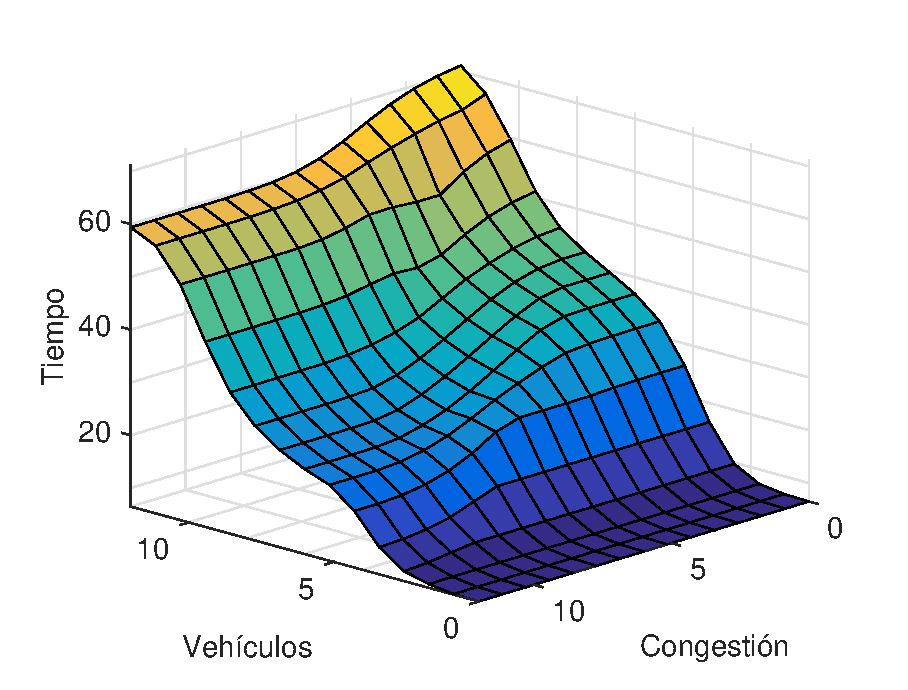
\includegraphics[width=11cm]{Surfaces/surface_d.eps}
	\captionof{figure}{Superficie de control del sistema de inferencia}
	\label{fig:surfaceControl}
\end{center}

\section{Comparativa de las superficies de control}
Las siguientes figuras son las curvas de control generadas por cada una de las configuraciones probadas en la sección \ref{section:desarrolloFIS}, cada una de las curvas representa, mediante una gráfica de 3 dimensiones (una superficie), los valores de salida obtenidos por las distintas configuraciones.

\begin{figure}[H]
	\centering
	\subfigure[Superficie A]{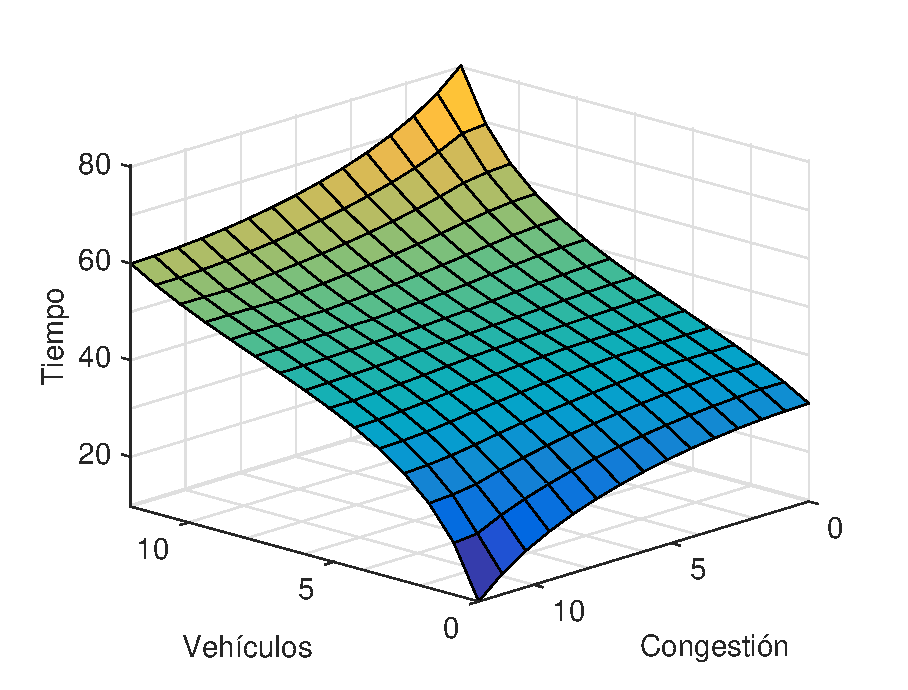
\includegraphics[width=8cm]{Surfaces/surface_a.eps}}
	\subfigure[Superficie B]{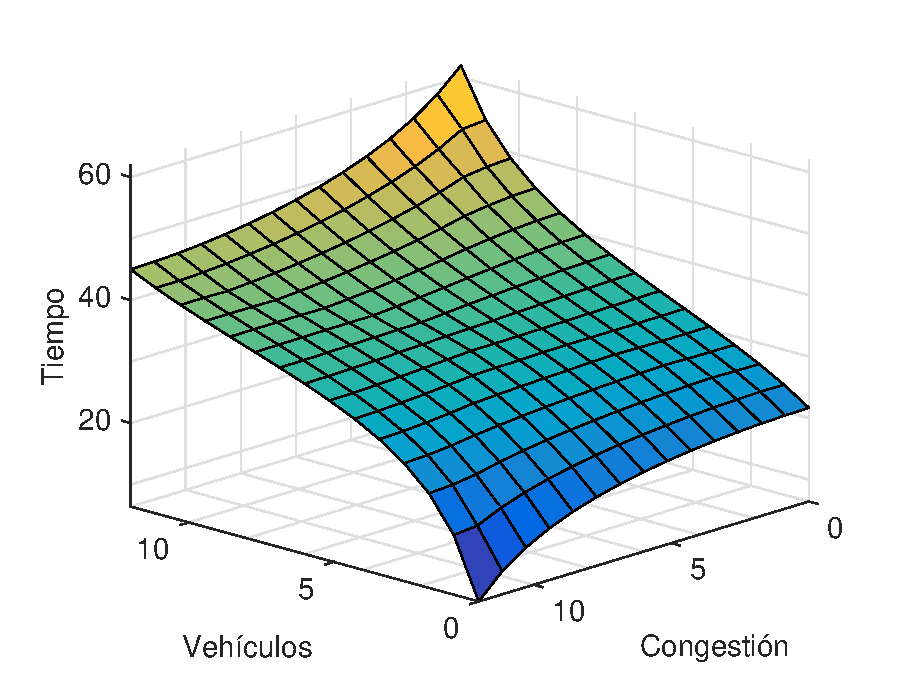
\includegraphics[width=8cm]{Surfaces/surface_b.eps}}
	\subfigure[Superficie C]{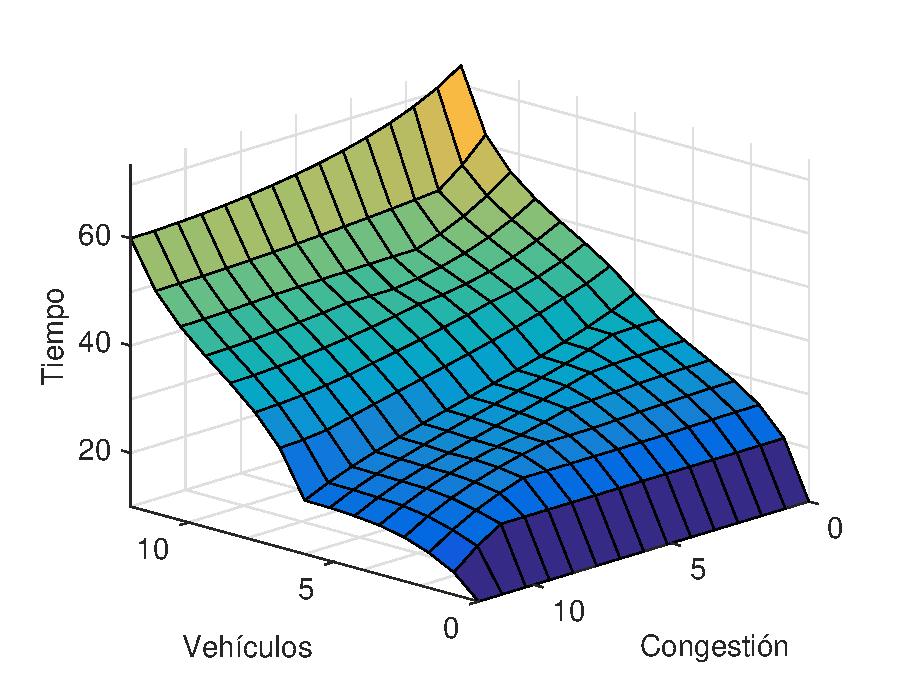
\includegraphics[width=8cm]{Surfaces/surface_c.eps}}
	\subfigure[Superficie D]{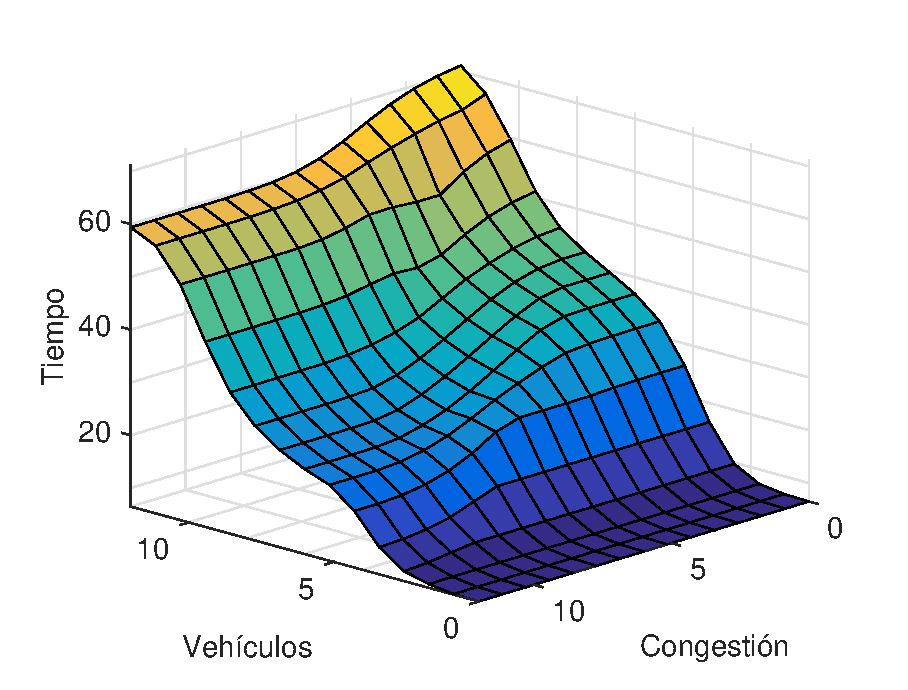
\includegraphics[width=8cm]{Surfaces/surface_d.eps}}
	\caption{Superficies de control}
\end{figure}

Las superficies mostradas arriba permiten ver el cambio gradual de las asignaciones de tiempo, de igual manera permiten apreciar la suavidad de la transición de los valores, además de que facilitan tener una perspectiva general de los valores de salida del sistema de inferencia.

Al analizar las gráficas se aprecia como las superficies A y B se ven afectadas de manera casi lineal por las variables de entrada. La diferencia más evidente es su rango de valores, pues la configuración A arroja valores de hasta 80s mientras que la B apenas rebasa los 60s.

En la superficie C se observa que existe un área donde la transición se vuelve un poco brusca e incluso toma una pendiente negativa. Este tipo de situaciones es más fácil observarlas cuando se recurre a una gráfica.

La superficie D, por otro lado, muestra una transición más limpia. También se observa como los valores de salida para congestiones altas se mantiene entre los 60s y 70s, mientras que para congestiones bajas se mantiene en un mínimo de alrededor de 10s.
Para valores de congestión entre 5 y 10, se observa como con los mismo valores para la variable vehículos, aumenta hasta alcanzar un máximo que se mantiene.

\section{Análisis de los repartos de tiempo}
Después de haber desarrollado y configurado la técnica seleccionada, ahora, en este capítulo se analizará el desempeño del algoritmo. Como se mencionó anteriormente, el algoritmo puede ser configurado para controlar intersecciones de diferente número de avenidas, carriles y avenidas. Con el fin de evaluar el desempeño del algoritmo frente a diferentes escenarios, se realizaron pruebas para los siguientes tipos de intersecciones que resultan ser las más comunes. 

{\setlength{\baselineskip}{0.5\baselineskip}
\begin{itemize}
	\item A: Intersecciones de 2 avenidas con 2 fases,
	\item B: Intersecciones de 4 avenidas con 2 fases y,
	\item C: Intersecciones de 4 avenidas con 4 fases.
\end{itemize}}

\textbf{Intersección A: 2 avenidas con 2 fases} Se entiende un cruce de dos calles de un solo sentido, donde el semáforo se encarga de ceder el paso de una sola de ellas en cada una de las fases (2 fases) tal y como se ve en la figura siguiente.
\begin{figure}[H]
	\centering
	\subfigure[Fase 1]{
	\begin{tikzpicture}[>=Triangle,scale=0.4]
		\clip (-4.5,4.5) rectangle (4.5,-4.5);	
		%calle eje x
		\fill[gray!50!white] (-4.5,1.5) rectangle (4.5,-1.5);
		%calle eje y
		\fill[gray!50!white] (-1.5,-4.5) rectangle (1.5,4.5);
		%semaforo
		\fill[black,scale=0.5] (3.35,1) rectangle (4,-1);
		\fill[black!30!red, scale=0.5] (3.65,0.65) circle(0.30);
		\fill[black!10!yellow, scale=0.5] (3.65,0) circle(0.30);
		\fill[black!60!green, scale=0.5] (3.65,-0.65) circle(0.30);
		%sentidos de las calles
		\draw[line width=0.6mm,->] (-4.5,0) -- (1.5,0);
		\draw [line width=0.6mm,->](-1.5,0) .. controls (0,0) and (0,0) .. (0,-3);
	\end{tikzpicture}
	}
	\subfigure[Fase 2]{
	
	\begin{tikzpicture}[>=Triangle,scale=0.4, rotate = 270]
		\clip (-4.5,4.5) rectangle (4.5,-4.5);
		%calle eje x
		\fill[gray!50!white] (-4.5,1.5) rectangle (4.5,-1.5);
		%calle eje y
		\fill[gray!50!white] (-1.5,-4.5) rectangle (1.5,4.5);
		%semaforo
		\fill[black,scale=0.5] (3.35,1) rectangle (4,-1);
		\fill[black!30!red, scale=0.5] (3.65,0.65) circle(0.30);
		\fill[black!10!yellow, scale=0.5] (3.65,0) circle(0.30);
		\fill[black!60!green, scale=0.5] (3.65,-0.65) circle(0.30);		
		%sentidos de las calles
		\draw[line width=0.6mm,->] (-4.5,0) -- (1.5,0);
		\draw [line width=0.6mm,->](-1.5,0) .. controls (0,0) and (0,0) .. (0,3);	
	\end{tikzpicture}
	}
	\caption{Intersección de 2 avenidas y 2 fases}
\end{figure}

\textbf{Intersección B: 4 avenidas con 2 fases.}
Se entiende un cruce de dos calles con doble sentido, donde el semáforo se encarga de ceder el paso a dos de ellas a la vez en cada fase, tal y como se ve en la figura siguiente. Normalmente se permite la vuelta a la izquierda con precaución.
\begin{figure}[H]
	\centering
	\subfigure[Fase 1]{
		\begin{tikzpicture}[>=Triangle,scale=0.4]
		\clip (-4.5,4.5) rectangle (4.5,-4.5);
		%calle eje x
		\fill[gray!50!white] (-4.5,1.5) rectangle (4.5,-1.5);
		%calle eje y
		\fill[gray!50!white] (-1.5,-4.5) rectangle (1.5,4.5);
		%semaforo
		\fill[black,scale=0.5] (-0.35,1) rectangle (0.35,-1);
		\fill[black!30!red, scale=0.5] (0,0.65) circle(0.30);
		\fill[black!10!yellow, scale=0.5] (0,0) circle(0.30);
		\fill[black!60!green, scale=0.5] (0,-0.65) circle(0.30);
		%division calles
		\draw [dashed,white,very thick] (-4.5,0) -- (-1.5,0);
		\draw [dashed,white,very thick] (6,1.5) -- (9,1.5);
		\draw [dashed,white,very thick] (0,4.5) -- (0,1.5);
		\draw [dashed,white,very thick] (0,-1.5) -- (0,-4.5);
		\draw [dashed,white,very thick] (1.5,0) -- (4.5,0);
		%sentidos de las calles
		\draw[line width=0.6mm,->] (-4.5,-0.75) -- (1.5,-0.75);
		\draw [line width=0.6mm,->](-1.5,-0.75) .. controls (-0.75,-0.75) and (-0.75,-0.75) .. (-0.75,-3);
		
		\draw[line width=0.6mm,->] (4.5,0.75) -- (-1.5,0.75);
		\draw [line width=0.6mm,->](1.5,0.75) .. controls (0.75,0.75) and (0.75,0.75) .. (0.75,3);
		\end{tikzpicture}
	}
	\subfigure[Fase 2]
	{
		\begin{tikzpicture}[>=Triangle, rotate= 90, scale=0.4]
		\clip (-4.5,4.5) rectangle (4.5,-4.5);
		%calle eje x
		\fill[gray!50!white] (-4.5,1.5) rectangle (4.5,-1.5);
		%calle eje y
		\fill[gray!50!white] (-1.5,-4.5) rectangle (1.5,4.5);
		%semaforo
		\fill[black,scale=0.5] (-0.35,1) rectangle (0.35,-1);
		\fill[black!30!red, scale=0.5] (0,0.65) circle(0.30);
		\fill[black!10!yellow, scale=0.5] (0,0) circle(0.30);
		\fill[black!60!green, scale=0.5] (0,-0.65) circle(0.30);
		%division calles
		\draw [dashed,white,very thick] (-4.5,0) -- (-1.5,0);
		\draw [dashed,white,very thick] (6,1.5) -- (9,1.5);
		\draw [dashed,white,very thick] (0,4.5) -- (0,1.5);
		\draw [dashed,white,very thick] (0,-1.5) -- (0,-4.5);
		\draw [dashed,white,very thick] (1.5,0) -- (4.5,0);
		%sentidos de las calles
		\draw[line width=0.6mm,->] (-4.5,-0.75) -- (1.5,-0.75);
		\draw [line width=0.6mm,->](-1.5,-0.75) .. controls (-0.75,-0.75) and (-0.75,-0.75) .. (-0.75,-3);
		
		\draw[line width=0.6mm,->] (4.5,0.75) -- (-1.5,0.75);
		\draw [line width=0.6mm,->](1.5,0.75) .. controls (0.75,0.75) and (0.75,0.75) .. (0.75,3);
		\end{tikzpicture}		
	}
	\caption{Intersección de 4 avenidas y 2 fases}
\end{figure}

\textbf{Intersección A: 4 avenidas con 2 fases.}
Se entiende un cruce de dos calles con doble sentido, donde el semáforo se encarga de ceder el paso a solo una de ellas en cada fase, tal y como se ve en la figura siguiente.
\begin{figure}[H]
	\centering
	\subfigure[Fase 1]
	{
		\begin{tikzpicture}[>=Triangle, scale=0.4]
		\clip (-4.5,4.5) rectangle (4.5,-4.5);
		%calle eje x
		\fill[gray!50!white] (-4.5,1.5) rectangle (4.5,-1.5);
		%calle eje y
		\fill[gray!50!white] (-1.5,-4.5) rectangle (1.5,4.5);
		%semaforo
		\fill[black,scale=0.5] (3.35,1) rectangle (4,-1);
		\fill[black!30!red, scale=0.5] (3.65,0.65) circle(0.30);
		\fill[black!10!yellow, scale=0.5] (3.65,0) circle(0.30);
		\fill[black!60!green, scale=0.5] (3.65,-0.65) circle(0.30);
		%division calles
		\draw [dashed,white,very thick] (-4.5,0) -- (-1.5,0);
		\draw [dashed,white,very thick] (6,1.5) -- (9,1.5);
		\draw [dashed,white,very thick] (0,4.5) -- (0,1.5);
		\draw [dashed,white,very thick] (0,-1.5) -- (0,-4.5);
		\draw [dashed,white,very thick] (2.5,0) -- (4.5,0);
		%sentidos de las calles
		\draw[line width=0.6mm,->] (-4.5,-0.75) -- (1.8,-0.75);
		\draw [line width=0.6mm,->](-1.5,-0.75) .. controls (-0.75,-0.75) and (-0.75,-0.75) .. (-0.75,-3);
		\draw [line width=0.6mm,->](-1.5,-0.75) .. controls (1,-0.75) and (1,-0.75) .. (1,3);
		\end{tikzpicture}		
	}
	\subfigure[Fase 2]
	{
		\begin{tikzpicture}[>=Triangle, scale=0.4, rotate=90]
		\clip (-4.5,4.5) rectangle (4.5,-4.5);
		%calle eje x
		\fill[gray!50!white] (-4.5,1.5) rectangle (4.5,-1.5);
		%calle eje y
		\fill[gray!50!white] (-1.5,-4.5) rectangle (1.5,4.5);
		%semaforo
		\fill[black,scale=0.5] (3.35,1) rectangle (4,-1);
		\fill[black!30!red, scale=0.5] (3.65,0.65) circle(0.30);
		\fill[black!10!yellow, scale=0.5] (3.65,0) circle(0.30);
		\fill[black!60!green, scale=0.5] (3.65,-0.65) circle(0.30);
		%division calles
		\draw [dashed,white,very thick] (-4.5,0) -- (-1.5,0);
		\draw [dashed,white,very thick] (6,1.5) -- (9,1.5);
		\draw [dashed,white,very thick] (0,4.5) -- (0,1.5);
		\draw [dashed,white,very thick] (0,-1.5) -- (0,-4.5);
		\draw [dashed,white,very thick] (2.5,0) -- (4.5,0);
		%sentidos de las calles
		\draw [line width=0.6mm,->] (-4.5,-0.75) -- (1.8,-0.75);
		\draw [line width=0.6mm,->](-1.5,-0.75) .. controls (-0.75,-0.75) and (-0.75,-0.75) .. (-0.75,-3);
		\draw [line width=0.6mm,->](-1.5,-0.75) .. controls (1,-0.75) and (1,-0.75) .. (1,3);
		\end{tikzpicture}
	}
	\subfigure[Fase 3]
	{
		\begin{tikzpicture}[>=Triangle, scale=0.4, rotate=180]
		\clip (-4.5,4.5) rectangle (4.5,-4.5);
		%calle eje x
		\fill[gray!50!white] (-4.5,1.5) rectangle (4.5,-1.5);
		%calle eje y
		\fill[gray!50!white] (-1.5,-4.5) rectangle (1.5,4.5);
		%semaforo
		\fill[black,scale=0.5] (3.35,1) rectangle (4,-1);
		\fill[black!30!red, scale=0.5] (3.65,0.65) circle(0.30);
		\fill[black!10!yellow, scale=0.5] (3.65,0) circle(0.30);
		\fill[black!60!green, scale=0.5] (3.65,-0.65) circle(0.30);
		%division calles
		\draw [dashed,white,very thick] (-4.5,0) -- (-1.5,0);
		\draw [dashed,white,very thick] (6,1.5) -- (9,1.5);
		\draw [dashed,white,very thick] (0,4.5) -- (0,1.5);
		\draw [dashed,white,very thick] (0,-1.5) -- (0,-4.5);
		\draw [dashed,white,very thick] (2.5,0) -- (4.5,0);
		%sentidos de las calles
		\draw [line width=0.6mm,->] (-4.5,-0.75) -- (1.8,-0.75);
		\draw [line width=0.6mm,->](-1.5,-0.75) .. controls (-0.75,-0.75) and (-0.75,-0.75) .. (-0.75,-3);
		\draw [line width=0.6mm,->](-1.5,-0.75) .. controls (1,-0.75) and (1,-0.75) .. (1,3);
		\end{tikzpicture}
	}
	\subfigure[Fase 4]
	{
		\begin{tikzpicture}[>=Triangle, scale=0.4, rotate=270]
		\clip (-4.5,4.5) rectangle (4.5,-4.5);
		%calle eje x
		\fill[gray!50!white] (-4.5,1.5) rectangle (4.5,-1.5);
		%calle eje y
		\fill[gray!50!white] (-1.5,-4.5) rectangle (1.5,4.5);
		%semaforo
		\fill[black,scale=0.5] (3.35,1) rectangle (4,-1);
		\fill[black!30!red, scale=0.5] (3.65,0.65) circle(0.30);
		\fill[black!10!yellow, scale=0.5] (3.65,0) circle(0.30);
		\fill[black!60!green, scale=0.5] (3.65,-0.65) circle(0.30);
		%division calles
		\draw [dashed,white,very thick] (-4.5,0) -- (-1.5,0);
		\draw [dashed,white,very thick] (6,1.5) -- (9,1.5);
		\draw [dashed,white,very thick] (0,4.5) -- (0,1.5);
		\draw [dashed,white,very thick] (0,-1.5) -- (0,-4.5);
		\draw [dashed,white,very thick] (2.5,0) -- (4.5,0);
		%sentidos de las calles
		\draw [line width=0.6mm,->] (-4.5,-0.75) -- (1.8,-0.75);
		\draw [line width=0.6mm,->](-1.5,-0.75) .. controls (-0.75,-0.75) and (-0.75,-0.75) .. (-0.75,-3);
		\draw [line width=0.6mm,->](-1.5,-0.75) .. controls (1,-0.75) and (1,-0.75) .. (1,3);
		\end{tikzpicture}
	}
	\caption{Intersección de 4 avenidas y 4 fases.}
\end{figure}



\textbf{Para cada una de las intersecciones} se suministra un conjunto de valores de prueba. Los valores inferidos por el algoritmo son presentados a manera de tablas en las siguientes secciones.





\newpage
\subsection{Intersección de 2 avenidas y 2 fases}
La siguiente tabla muestra los valores (aleatorios) de entrada suministrados para cada una de las 4 pruebas realizadas, cada uno de los valores representa la cantidad de autos por avenida. Además, se observa el número de carriles de cada avenida y las avenidas que intervienen en cada \emph{fase en verde}.

\begin{longtable}[c]{ccccc} \toprule
	\textbf{No} &\multicolumn{2}{c}{\textbf{Vehículos}} & \multicolumn{2}{c}{\textbf{Tiempos asignados}} \\[0.2cm]
	&  Avenida 1 & Avenida 2 & Fase 1 & Fase 2 \\[0cm]
	&{\scriptsize(1 carril)}&{\scriptsize (1 carril)} &{\scriptsize (av 1)} &{\scriptsize(av 2)} \\[0.1cm]\midrule
	1 & 1 & 8 & 8.58 &43.09\\
	3 & 4 & 7 & 22.29 & 35.74\\
	2 & 12 & 5 & 61.69 & 21.40\\
	4 & 12 & 10 & 59.39 & 48.29\\\bottomrule
	\caption{Valores de prueba para la intersección A}
\end{longtable}

Las siguientes gráficas representan los repartos de tiempo para cada conjunto de valores de prueba. A diferencia de una asignación estática, aquí se observa como los tiempos varían en función de la cantidad de vehículos.

\begin{figure}[H]
	\centering
	\subfigure[Prueba No. 1]{\begin{tikzpicture}[scale=0.4]\pie[style=drop shadow, sum=auto, text=legend, after number={s}, cloud]{8.6/{Fase 1}, 43.1/{Fase 2} } \end{tikzpicture} }
	\subfigure[Prueba No. 2]{\begin{tikzpicture}[scale=0.4]\pie[style=drop shadow, sum=auto, text=legend, after number={s}, cloud]{22.3/{Fase 1}, 35.7/{Fase 2} } \end{tikzpicture} }\\
	\subfigure[Prueba No. 3]{\begin{tikzpicture}[scale=0.4]\pie[style=drop shadow, sum=auto, text=legend, after number=s, cloud]{61.7/{Fase 1}, 21.4/{Fase 2} } \end{tikzpicture} }
	\subfigure[Prueba No. 4]{\begin{tikzpicture}[scale=0.4]\pie[style=drop shadow, sum=auto, text=legend, after number=s, cloud]{59.4/{Fase 1}, 48.3/{Fase 2} } \end{tikzpicture} }
	\caption{Repartos de tiempo de la intersección A}
\end{figure}





\newpage
\subsection{Intersección de 4 avenidas y 2 fases}
Al igual que en la sección anterior, se observa los valores de prueba suministrados y los tiempos inferidos por el sistema de inferencia, también se observa el número de carriles de cada avenida y las avenidas que intervienen en cada \emph{fase en verde}.
\begin{longtable}[c]{ccccccc} \toprule
	\textbf{No} &\multicolumn{4}{c}{\textbf{Vehículos}} & \multicolumn{2}{c}{\textbf{Tiempos asignados}} \\[0.2cm]
	&  Avenida 1 & Avenida 2 &  Avenida 3 & Avenida 4 & Fase 1 & Fase 2 \\[0cm]
	&{\scriptsize(2 carriles)}&{\scriptsize (1 carril)} &{\scriptsize (2 carriles)} & {\scriptsize (1 carril)} &{\scriptsize (avs 1 y 3)} &{\scriptsize(avs 1 y 4)} \\[0.1cm]\midrule
	1 & 1 & 8 & 8 & 10 & 9.45 &45.68\\
	3 & 2 & 4 & 8 & 12 & 9.45 & 42.04\\
	2 & 20 & 10 & 12 & 5 & 31.53 & 27.09\\
	4 & 30 & 12 & 7 & 5 & 37.76& 30.86 \\\bottomrule
	\caption{Valores de prueba para la intersección B}
\end{longtable}

Las siguientes gráficas representan los repartos de tiempo para cada conjunto de valores de prueba.
\begin{figure}[H]
	\centering
	\subfigure[Prueba No. 1]{\begin{tikzpicture}[scale=0.4]\pie[style=drop shadow, sum=auto, text=legend, after number={s}, cloud]{9.45/{Fase 1}, 45.68/{Fase 2} } \end{tikzpicture} }
	\subfigure[Prueba No. 2]{\begin{tikzpicture}[scale=0.4]\pie[style=drop shadow, sum=auto, text=legend, after number={s}, cloud]{9.45/{Fase 1}, 42.04/{Fase 2} } \end{tikzpicture} }\\
	\subfigure[Prueba No. 3]{\begin{tikzpicture}[scale=0.4]\pie[style=drop shadow, sum=auto, text=legend, after number=s, cloud]{31.53/{Fase 1}, 27.09/{Fase 2} } \end{tikzpicture} }
	\subfigure[Prueba No. 4]{\begin{tikzpicture}[scale=0.4]\pie[style=drop shadow, sum=auto, text=legend, after number=s, cloud]{37.76/{Fase 1}, 30.86/{Fase 2} } \end{tikzpicture} }
	\caption{Repartos de tiempo de la intersección B}
\end{figure}




\newpage
\subsection{Intersección de 4 avenidas y 4 fases}
Al igual que en las secciones anteriores, se observa los valores de prueba suministrados y los tiempos inferidos, también se observa el número de carriles de cada avenida y las avenidas que intervienen en cada \emph{fase en verde}.

\begin{longtable}[c]{ccccccccc} \toprule
	\textbf{No} & \multicolumn{4}{c}{\textbf{Vehículos}} & \multicolumn{4}{c}{\textbf{Tiempos asignados}} \\[0.2cm]
	
	&  Avenida 1 & Avenida 2 &  Avenida 3 & Avenida 4 & Fase 1 & Fase 2 & Fase 3 & Fase 4\\[0cm]
	
	&{\scriptsize(3 carriles)}&{\scriptsize (2 carriles)}
	&{\scriptsize(2 carriles)}&{\scriptsize (1 carril)}
	&{\scriptsize (av 1)} &{\scriptsize(av 2)}
	&{\scriptsize (av 3)} &{\scriptsize(av 2)} \\[0.1cm]\midrule
	
	1 & 2 	& 8		& 8 	& 10 	& 08.44 & 22.43 & 22.43 & 52.65 \\
	3 & 2 	& 4 	& 8 	& 12 	& 08.44 & 09.45 & 22.43 & 70.07 \\
	2 & 20 	& 10 	& 12 	& 5 	& 31.42 & 28.09 & 31.52 & 28.09\\
	4 & 30 	& 12	& 7 	& 5 	& 49.76 & 26.63 & 13.28 & 25.59 \\\bottomrule
	\caption{Valores de prueba para la intersección C}
\end{longtable}

El reparto de tiempos es el siguiente:
\begin{figure}[H]
	\centering
	\subfigure[Prueba No. 1]{\begin{tikzpicture}[scale=0.5]\pie[style=drop shadow, sum=auto, text=legend, after number={s}, cloud]
		{8.4/{Fase 1}, 22.4/{Fase 2}, 22.4/{Fase 3}, 52.7/{Fase 4} } \end{tikzpicture} }
	\subfigure[Prueba No. 2]{\begin{tikzpicture}[scale=0.5]\pie[style=drop shadow, sum=auto, text=legend, after number={s}, cloud]
		{8.4/{Fase 1}, 9.5/{Fase 2}, 22.4/{Fase 3}, 70.1/{Fase 4} } \end{tikzpicture} }\\
	\subfigure[Prueba No. 3]{\begin{tikzpicture}[scale=0.5]\pie[style=drop shadow, sum=auto, text=legend, after number={s}, cloud]
		{31.4/{Fase 1}, 28.1/{Fase 2}, 31.5/{Fase 3}, 28.1/{Fase 4} } \end{tikzpicture} }
	\subfigure[Prueba No. 4]{\begin{tikzpicture}[scale=0.5]\pie[style=drop shadow, sum=auto, text=legend, after number={s}, cloud]
		{49.8/{Fase 1}, 26.6/{Fase 2}, 13.3/{Fase 3}, 25.6/{Fase 4} } \end{tikzpicture} }
	\caption{Repartos de tiempo de la intersección C}
\end{figure}


\include{Capitulo_06}

% Apendices
\appendix
\chapter{Diagramas de clases UML}\label{apendice:a}
En la sección \ref{subsection:umlclases}, página \pageref{subsection:umlclases} se mostró el siguiente diagrama UML con elementos omitidos, ahora se presentarán el resto de diagramas completos.

\begin{figure*}[h]
	\begin{tikzpicture}
	
	\umlsimpleclass[y=-2.5]{MySemaforo}
	\umlsimpleclass[x=-6.6, y=0]{FuzzySet}
	\umlsimpleclass[x=6.5, y=-2.5]{MySensor}
	\umlsimpleclass[type=abstract]{FuzzySemaforo}
	
	\umlsimpleclass[x=-4, y=3.5]{TriangularMF}
	\umlsimpleclass[x=0, y=3.5]{SigmoidalMF}
	\umlsimpleclass[x=4, y=3.5]{GaussianaMF}
	
	\umlsimpleclass[x=-6.6, y=7]{FuzzyValue}
	\umlsimpleclass[x=0, y=7, type=abstract]{MembershipFunction}
	\umlsimpleclass[x=6.5, y=7, type=abstract]{SensorVehiculos}
	
	\umlunicompo[geometry=|-|, anchor1=140, mult1=1, mult2=0..*, pos2=2.8]{FuzzySemaforo}{TriangularMF}
	\umlunicompo[geometry=|-|, anchor1=90, mult1=1, mult2=0..*, pos2=2.8]{FuzzySemaforo}{SigmoidalMF}
	\umlunicompo[geometry=|-|, anchor1=40, mult1=1, mult2=0..*, pos2=2.8]{FuzzySemaforo}{GaussianaMF}
	
	\umlunicompo[mult1=1, pos1=0, align1=right, mult2=0..*, pos2=1, align2=left]{FuzzySemaforo}{FuzzySet}
	\umluniassoc[geometry=-|, anchor2=-130, attr2=cuenta vehículos|1, pos2=1, align2=right, align1=left, mult1=1, pos1=0]{FuzzySemaforo}{SensorVehiculos}
	\umlimpl[geometry=|-|]{TriangularMF}{MembershipFunction}
	\umlimpl[geometry=|-|]{SigmoidalMF}{MembershipFunction}
	\umlimpl[geometry=|-|]{GaussianaMF}{MembershipFunction}
	
	\umlimpl{MySensor}{SensorVehiculos}
	\umluniassoc[mult1=1, pos1=0, align1=right, mult2=0..1, pos2=1, align2=left]{MembershipFunction}{FuzzyValue}
	\umluniassoc[mult1=1, pos1=0.05, mult2=0..1, pos2=1, align2=left]{FuzzySet}{FuzzyValue}	
	
	\umlimpl{MySemaforo}{FuzzySemaforo}
	\end{tikzpicture}
	\caption{Diagrama de clases que muestra las relaciones del sistema}
	\label{uml:relaciones2}
\end{figure*}
\newpage

\section{Diagramas de las clases \textit{FuzzySet y FuzzyValue}}

\begin{figure}[H]
	\centering
	\begin{tikzpicture}
	
	\umlclass[anchor=north, y=-4]
	{FuzzySet}
	{- set\_u : vector< double > \\- set\_x : vector< double >}
	{+ FuzzySet( begin : double, step : double, end : double )\\
		+ FuzzySet( set : FuzzySet, f : MembershipFunction)\\
		+ operator>>( a : FuzzySet, b : FuzzySet) : FuzzySet\\
		+ operator\&( a : FuzzySet, b : FuzzySet) : FuzzySet\\
		%  	 + Print(show\_cero : bool ) : void \\
		+ get\_centroid() : double}
	
	\umlclass[]
	{FuzzyValue}
	{- x : double}
	{+ FuzzyValue( x : double) \\
		+ FuzzyValue( v : FuzzyValue)\\
		+ operator\_double() : double\\
		+ operator=( v : FuzzyValue) : FuzzyValue\\
		+ operator\&( v : FuzzyValue ) : FuzzyValue}
	\end{tikzpicture}
	\caption{Diagrama de las clases \emph{FuzzySet} y \emph{FuzzyValue}}
\end{figure}
\newpage

\section{Jerarquía de herencia \textit{MembershipFunction}}
El siguiente diagrama UML modela los miembros de las clases \textit{MembershipFunction, TriangularMF, SigmoidalMF, GaussianaMF}, además muestra su relación de herencia.


\begin{figure}[h]
	\centering
	\begin{tikzpicture}
	\umlclass[type=abstract]{MembershipFunction}{}{\umlvirt{+ operator()( x : double ) : FuzzyValue}}
	
	\umlclass[x=8.1, y=5]
	{TriangularMF}
	{- a : double\\- b : double\\- c : double}
	{+ TriangularMF( a : double, b : double, c : double )\\+ operator()( x : double ) : FuzzyValue }
	
	\umlclass[x=9, y=0]
	{SigmoidalMF}
	{- a : double\\- $x_0$ : double}
	{+ SigmoidalMF( a : double, $x_0$ : double )\\+ operator()( x : double ) : FuzzyValue }
	
	\umlclass[x=9, y=-5]
	{GaussianaMF}
	{- a : double\\- $x_0$ : double}
	{+ GaussianaMF( a : double, $x_0$ : double )\\+ operator()( x : double ) : FuzzyValue }
	
	\umlimpl[geometry=-|]{TriangularMF}{MembershipFunction}
	\umlimpl[]{SigmoidalMF}{MembershipFunction}
	\umlimpl[geometry=-|]{GaussianaMF}{MembershipFunction}
	\end{tikzpicture}
	\caption{Diagrama de clases que modela la jerarquía de herencia MembershipFunction }
\end{figure}


\newpage
\section{Realización de la clase \textit{SensorVehiculos}}
El siguiente diagrama modela los elementos omitidos de las clases \textit{SensorVehiculos} y \textit{MySensor}, además, se modela su relación de herencia y \emph{realización}.\\

\begin{figure}[h]
	\centering
	\begin{tikzpicture}
	\umlclass[type=abstract]
	{SensorVehiculos}
	{}
	{\umlvirt{+ read() : vector< double >} }
	
	\umlclass[y=-5]
	{MySensor}
	{ - num\_camaras : int }
	{ + SensorGenerico( camaras : int ) \\ + read() : vector< double > }
	
	\umlimpl[]{MySensor}{SensorVehiculos}
	
	\umlnote[x=-7, y=-5, anchor2=-160, width=4cm]{MySensor}{Esta clase es solo para demostración, deberá ser implementada adecuadamente por el usuario final }
	\end{tikzpicture}
	\caption{Diagrama de clases que modela la implementación de \textit{SensorVehiculos:read()}}
\end{figure}


\newpage
\section{Realización de la clase \textit{FuzzySemaforo}}
El siguiente diagrama modela los elementos omitidos de las clases \textit{FuzzySemaforo} y \textit{MySemaforo}, además, se modela su relación de herencia y \emph{realización}.\\

\begin{figure}[H]
	\centering
	\begin{tikzpicture}
	\umlclass[type=abstract]
	{FuzzySemaforo}
	{- num\_fases : int\\
		- num\_carriles : int\\
		- num\_avenidas : int\\
		- fase : int \\
		- tiempo : double\\
		- vehiculos : double\\
		- congestion : double\\
		- autos : vector< double >\\
		- pesos : vector< double >\\
		- ciclo : Ciclo\\
		- carriles : Carril\\
		- sensor : SensorVehiculos}
	{+ FuzzySemaforo( ciclo:Ciclo, carril:Carril, sensor:SensorVehiculos )\\
		+ run() : void\\
		\umlvirt{+ set\_lights( fase : int, tiempo : double ) : void}\\
		- get\_time( t : int, c : int) : double\\
		- get\_media( fase : int, estado : int)}	
	
	\umlclass[y=-9]{MySemaforo}{}
	{+ MySemaforo(ciclo:Ciclo, carriles:carril, sensor:SensorVehiculos)\\
		+ set\_lights( fase : int, tiempo : double) : void}
	
	\umlimpl{MySemaforo}{FuzzySemaforo}
	\umlnote[x=-8, y=-9, width=3cm]{MySemaforo}{Esta clase es solo para demostración, deberá ser implementada adecuadamente por el usuario final }
	\end{tikzpicture}
	\caption{Diagrama de clases que modela la implementación de \textit{set\_lights: FuzzySemaforo}}
\end{figure}

\chapter[Algoritmo de detección de vehículos]{Implementación en C++ de un algoritmo de detección de vehículos}\label{apendice:b}
Del resultado de la investigación realizada en \cite{ittap} se rescata el algoritmo de visión computacional seleccionado para la detección de automóviles. Dicho trabajo arroja un algoritmo implementado en \emph{Python} que, según los resultados de la propia investigación, ha probado tener una eficacia (con buena iluminación) de hasta un 95\%.

El tiempo de ejecución del algoritmo sugerido por \emph{Estrada \& Recinos \& Vidal (2017)}: ``Detección de vehículos mediante imagen de fondo '' es de 1.5 segundos (implementado en Python), sin embargo al implementarse en C++ alcanza un tiempo de 0.03 segundos, es decir, 3 centésimas de segundo. 

\textbf{Requerimientos}\\
El algoritmo en su versión C++ requiere de un compilador que soporte el estándar ISO C++11 además de tener compilado e instalado la librería para visión por computadora OpenCV en su versión 2.x. \\\\
\textbf{Código Fuente}\\
\lstinputlisting[
style=ezam,
caption={[Implementación en C++] Implementación en C++ del algoritmo de detección de vehículos}
]{algoritmo.cpp}


% Bibliografia
\begin{thebibliography}{99}
	
	\bibitem{garciag} García, G. (2017). Un enfoque de semáforo inteligente utilizando algoritmos de visión computacional en una intersección aislada para optimizar el flujo vehicular (Tesis de maestría). Centro de Investigación en Inteligencia Artificial (CIIA) de la Universidad Veracruzana, Xalapa de Enríquez, Veracruz, México. 
	
	\bibitem{alvaroer} Alvaro E., R. De Somocurcio S. (2008). Control de tráfico vehicular automatizado utilizando Lógica Difusa. Universidad Ricardo Palma, Lima, Perú.
	
	\bibitem{bencesramos} Bances, M., Ramos, M. (2014). Semáforos Inteligentes para la regulación del tráfico vehicular. Rev. Ingeniería: Ciencia, Tecnología e Innovación. Vol. 1 (No. 1). pp. 37-45. .
	
	\bibitem{MoraleslGonzales} Morales, L. Rafael., Gonzáles, S. Juan. (2013) \emph{Control de tráfico vehicular por medio de semáforos inteligentes}. Universidad de Rafael Urdaneta, República Bolivariana de Venezuela.  
	
	\bibitem{Hernandezca} Hernández, C.A., Salcedo, O., \& Pedraza, L.F. (2007). Modelo de Semaforización Inteligente para la Ciudad de Bogotá. Revista Científica y Tecnológica de la Facultad de Ingeniería, Universidad Distrital Francisco José de Caldas, Vol. 11(No.2). 61-69. 
	
	\bibitem{ittap} Estrada, E.K., Recinos, H., \& Vidal, G. Y. (2017). Selección de un algoritmo de visión por computadora para la detección de vehículos. Instituto Tecnológico de Tapachula, Tapachula, Chiapas, México.
	
	\bibitem{duarte} Oscar G. Duarte (1999). Sistemas de lógica difusa. Fundamentos. \textit{Revista Ingeniería e Investigación, No. 42, pp. 22.}
	
	\bibitem{sedesolpa} Secretaría de Desarrollo Social (SEDESOL). (1994). Programa de Asistencia técnica en transporte urbano para las ciudades medias mexicanas. Manual Normativo, Tomo XII. Estudios de Ingeniería de Tránsito. México.
	
	\bibitem{minusterioti} Ministerio de Transporte e Infraestructura. (2008). Manual para la Revisión de Estudios de Tránsito. Realización de Manuales Técnicos para la Revisión y Aprobación de Estudios y Diseños de Carreteras. Managua, Nicaragua.
	
	\bibitem{arandia} Juan Gabriel Tapia Arandia, Romel Daniel Veizaga Balta (2006).
		\emph{Apoyo didáctico para la enseñanza y aprendizaje de la asignatura de ingeniería de tráfico}.
		(Trabajo para optar al diploma de Licenciatura en Ingeniería Civil).
		Universidad Mayor De San Simón, Cochabamba, Bolivia.
	
	\bibitem{zadehfs} Zadeh, A.L. (1965). Fuzzy sets \emph{Information and Control}, vol. 8, pp. 338-353.
	
	\bibitem{zadehnewapproach} Zadeh, A.L. (1973). Outline of a New Approach to the Analysis of Complex Systems and Decision Processes. \emph{IEEE Transactions on Systems, Man, and Cybernetics}, Vol. SMC-3, (No. 1). 28-44.
	
	\bibitem{zadehlinguisticv} Zadeh, A.L. (1975). The Concept of a Linguistic Variable and its Application to Approximate Reasoning-I. \emph{Information Sciences}. Vol. 8. 199-249.
	
	\bibitem{ponce} Ponce Cruz P. (Primera Edición). (2010).
		\emph{Inteligencia Artificial con Aplicaciones a la Ingeniería}. México: Alfaomega.
	
	\bibitem{amador} Amador Hidalgo L. (Primera Edición). (1997).
		\emph{Inteligencia Artificial y Sistemas Expertos}. Córdoba: Universidad de Córdoba.
		
	\bibitem{alfonsovr2013} Alfonso V. Rivera. (2013). \emph{Controladores difusos aplicados a convertidores DC/DC} (Tesis de maestría). Universidad Autónoma de Aguascalientes, Aguascalientes, Ags.
	
	\bibitem{carlosgm} Carlos G. Morcillo. \emph{Lógica Difusa, una introducción práctica}. E-mail: Carlos.Gonzales@uclm.es
	
	\bibitem{josecarlos} José Carlos. \emph{Control Neuro-Difuso Aplicado a una Grúa Torre}. Recuperado de Tesis Digitales UNMSM
	
	\bibitem{kevinstephe} Kevin M. Passino, Stephen Yurkovick, (1997). \emph{Fuzzy Control}. California, Berkeley: ADDISON-WESLEY
	
	\bibitem{MarinIA} Marín, M. R., Palma, M. J. (2008). Inteligencia Artificial: Métodos, técnicas y aplicaciones. España: Mcgraw-Hill/Interamericana De España, S. A. U.
	\bibitem{IssaiGalvan} Isasi, V. P., Galván, L. I. (2004). Redes de Neuronas Artificiales: Un enfoque práctico. Madrid, España: Pearson Educación, S.A.
	
\end{thebibliography}



\end{document}